\documentclass[a4paper]{article}
\usepackage{geometry}
\geometry{
	a4paper,
	total={170mm,257mm},
	left=27mm,
	right=30mm,
	top=30mm,
	bottom= 30mm
}
\usepackage{lipsum}
\usepackage{tabu}
\usepackage[english]{babel}
\usepackage[utf8]{inputenc}
\usepackage[parfill]{parskip}
\usepackage{longtable}
\usepackage{amsmath}
\usepackage{graphicx}
\usepackage{enumitem}
\usepackage[colorinlistoftodos]{todonotes}
\usepackage{tikz}
\newcommand*\circled[1]{\tikz[baseline=(char.base)]{
		\node[shape=circle,draw,inner sep=0.5pt] (char) {#1};}}
\usetikzlibrary{fit,positioning}
\usepackage{authblk}
\usepackage{natbib}
\usepackage[algo2e]{algorithm2e}
\usepackage{algorithmic}  
\usepackage{algorithm}
\usepackage{comment}
\usepackage{array}% http://ctan.org/pkg/array
\makeatletter
\g@addto@macro{\endtabular}{\rowfont{}}% Clear row font
\makeatother
\newcommand{\rowfonttype}{}% Current row font
\newcommand{\rowfont}[1]{% Set current row font
	\gdef\rowfonttype{#1}#1%
}
\newcolumntype{L}{>{\rowfonttype}l}
\title{A Network Model for Dynamic Textual Communications \\with Application to
	Government Email Corpora}
%\author{Bomin Kim}

\author[1]{Bomin Kim}
\author[3]{Aaron Schein}
\author[1]{Bruce Desmarais}
\author[2,3]{Hanna Wallach}
\affil[1]{Pennsylvania State University}
\affil[2]{Microsoft Research NYC}
\affil[3]{University of Massachusetts Amherst}

\begin{document}
\setlength{\parindent}{0pt}
\maketitle
\begin{abstract}
	
	\noindent In this paper, we introduce the interaction-partitioned topic model
	(IPTM)---a probabilistic model of who communicates with whom about
	what, and when. Broadly speaking, the IPTM partitions time-stamped
	textual communications, such as emails, according to both the network
	dynamics that they reflect and their content. To define the IPTM, we
	integrate a dynamic version of the exponential random graph model---a
	generative model for ties that tend toward structural features such as
	triangles---and latent Dirichlet allocation---a generative model for
	topic-based content. The IPTM assigns each topic to an "interaction
	pattern"---a generative process for ties that is governed by a set of
	dynamic network features. Each communication is then modeled as a
	mixture of topics and their corresponding interaction patterns. We use
	the IPTM to analyze emails sent between department managers in two
	county governments in North Carolina; one of these email corpora
	covers the Outer Banks during the time period surrounding Hurricane
	Sandy. Via this application, we demonstrate that the IPTM is effective
	at predicting and explaining continuous-time textual communications.
\end{abstract}
\section{Introduction} \label{sec: Introduction}


In recent decades, real-time digitized textual communication has developed into a ubiquitous form of social and professional interaction \citep[see, e.g.,][]{kanungo2008modeling, szostek2011dealing, burgess2004email, pew2016}. From the perspective of the computational social scientist, this has lead to a growing need for methods of modeling interactions that manifest as text exchanged in continuous time (e.g., e-mail messages). A number of models that build upon topic modeling through Latent Dirichlet Allocation \citep{Blei2003} to incorporate link data as well as textual content have been developed recently \citep{mccallum2005author,lim2013twitter,Krafft2012}. These models are innovative in their extensions that incorporate network tie information. However, none of the models that are currently available in the literature integrate the rich random-graph structure offered by state of the art models for network structure---in particular, the exponential random graph model (ERGM) \citep{robins2007introduction,chatterjee2013estimating,hunter2008ergm}. The ERGM is the canonical model for network structure, as it is flexible enough to specify a generative model that accounts for nearly any pattern of tie formation (e.g., tie reciprocation, clustering, popularity effects) \citep{desmarais2017statistical}. We build upon recent extensions of ERGM that model time-stamped ties \citep{PerryWolfe2012,Butts2008}, and develop the interaction-partitioned topic model (IPTM) to simultaneously model the network structural patterns that govern tie formation, and the content in the communications.

ERGM, and models based on ERGM, provide a framework for explaining or predicting ties between nodes using the network sub-structures in which the two nodes are embedded (e.g., an ERGM specification may predict ties between two nodes that have many shared partners). ERGM-style models have been used for many applications in which the ties between nodes are annotated with text. The text, despite providing rich information regarding the strength, scope, and character of the ties, has been largely excluded from these analyses, due to the inability of ERGM-style models to incorporate textual attributes of ties. These application domains include, among other applicaitons, the study of legislative networks in which networks reflect legislators' co-support of bills, but exclude bill text \citep{bratton2011networks,aleman2013explaining}; the study of alliance networks in which networks reflect countries' co-signing of treaties, but exclude treaty text \citep{camber2010geometry,cranmer2012complex,cranmer2012toward,kinne2016agreeing}; the study of scientific co-authorship networks that exclude the text of the co-authored papers \citep{kronegger2011collaboration,liang2015changing,fahmy2016gender}; and the study of text-based interaction on social media (e.g., users tied via `mentions' on twitter) \citep{yoon2014strategies,peng2016follower,lai2017connecting}.

In defining and testing the IPTM we embed three core conceptual properties, in addition to modeling both text and network structure. First, we link the content component of the model, and network component of the model such that knowing who is communicating with whom at what time (i.e., the network component) provides information about the content of communication,  and vice versa. Second, we fully specify the network dynamic component of the model such that, given the content of the communication and the history of tie formation, we can draw an exact, continuous-time prediction of when, by whom, and to whom the communication will be sent. Third, we formulate the network dynamic component of the model such that the model can represent, and be used to test hypotheses regarding, canonical processes relevant to network theory such as preferential attachment---the tendency for actors to prefer interacting with actors who have been popular in the past \citep{barabasi1999emergence,vazquez2003growing,jeong2003measuring}, reciprocity \citep{hammer1985implications,rao1987measures}, and transitivity---the tendency for the friends of friends to become friends \citep{louch2000personal,burda2004network}. In what follows we (1) present the generative process for the IPTM, describing how it meets our theoretical criteria, (2) derive the sampling equations for Bayesian inference with the IPTM, and (3) illustrate the IPTM through application to email corpora of internal communications by county officials in North Carolina county governments. {\bf [What predictive comparisons should we run to other models]}?

\section{IPTM: Model Definition and Derivation} \label{sec: Generative Process}

To define and derive the IPTM, we begin by describing a probabilistic process by which documents are generated, where documents include a sender, recipients, contents, and timing. We provide a fully parametric definition of each component of the generative process, which enables the model to be used to simulate distributions of who communicates with whom about what, and when. We take a Bayesian approach to inference for the parameters of the IPTM. In the next section, we derive equations for sampling from the posterior distributions of the IPTM parameters conditional on data generated by the generative process that we define in the current section.

The data generated under the IPTM consists of $D$ unique documents. A single email, indexed by $d \in \{1,...,D\}$, is represented by the four components ($i^{(d)}, J^{(d)}, t^{(d)},  \boldsymbol{w}^{(d)}$). The first two are the sender and recipients of the email: an integer $i^{(d)} \in \{1,...,A\}$ indicates the identity of the sender out of $A$ actors (or nodes) and an integer vector $J^{(d)} = \{j_r^{(d)}\}_{r=1}^{|J^{(d)}|} $, which indicates the identity of the receiver (or receivers) out of $A-1$ actors, where $|J^{(d)}|\in \{1,...,A-1\}$ denotes the total number of receivers. Next, $t^{(d)}$ is the  timestamp of the email $d$, and $\boldsymbol{w}^{(d)} = \{w^{(d)}_n \}_{n=1}^{N^{(d)}}$ is a set of tokens, or word type instances, that comprise the text of the email. In this section, we illustrate how the words $\boldsymbol{w}^{(d)}$ are generated according to latent Dirichlet allocation \citep{Blei2003}, and then how the other components, ($i^{(d)}, J^{(d)}, t^{(d)}$), are generated conditional on the document content. For simplicity, we assume that documents are ordered by time such that $t^{(d)} < t^{(d+1)}$ for all $d=1, ..., D$. 
\subsection{Content Generating Process} \label{subsec: Content Generating Process} 
The content generating process follows from the generative process of Latent Dirichlet Allocation \cite{Blei2003}. First we generate the global (corpus-wide) variables. Each topic $k$ is associated with a cluster, or interaction pattern, assignment $c_k$, where $c_k$ can take one of $c = \{1,2,...,C\}$ values.  There are two main sets of global variables---those that describe the content via topics and those that describe how people interact (interaction patterns). These variables are linked by a third set of variables that associate each topic with the pattern that best describes how people interact when talking about that topic. \newline
There are $K$ topics. Each topic $k$ is a discrete distribution over $V$ word types.
\begin{itemize}
	\item[1.] {$\boldsymbol{\phi}^{(k)} \sim \mbox{Dirichlet}(\beta, \bf u)$} \textbf{[See Algorithm 1]}\\
	- A topic $k$ is characterized by a discrete distribution over $V$ word types with probability vector $\phi^{(k)}$. We specify a symmetric Dirichlet prior $\bf u$ with the concentration parameter $\beta$ for the probability vector $\phi^{(k)}$.
\end{itemize}
\noindent There are $C$ interaction patterns. Each interaction pattern consists of a vector of coefficients $\boldsymbol{b}^{(c)}$ in $\boldsymbol{R}^{P}$ and a vector of P-dimensional dynamic network statistics for directed edge $(i, j)$ at time $t$ $\boldsymbol{x}^{(c)}_t(i, j)$. The inner product of $\boldsymbol{b}^{(c)}$ and $\boldsymbol{x}^{(c)}_t(i, j)$ is used to generate both the recipient vector for a document and the timing of the document.
\begin{itemize}
	\item[2.] $\boldsymbol{b}^{(c)}\sim \mbox{Multivariate Normal}(\mu_{\boldsymbol{b}}, \Sigma_{\boldsymbol{b}})$ \textbf{[See Algorithm 2]}: \\
		- The vector of coefficients depends on the interaction pattern $c$. This means that there is variation across interaction patterns in the degree to which document timing and recipients depend upon the dynamic network statistics. The prior for $\boldsymbol{b}^{(c)}$ is a P-variate multivariate Normal with mean vector $\mu_{\boldsymbol{b}}$ and covariance matrix $\Sigma_{\boldsymbol{b}}$.
	\end{itemize}
\noindent The topics and interaction patterns are tied together via a set of $K$ categorical variables.
\begin{itemize}
	\item[3.] $c_k\sim \mbox{Uniform}(1, C)$ \textbf{[See Algorithm 3]}: \\
	- Each topic is associated with a single interaction pattern.\\
\end{itemize}
\noindent We have now defined all of the variables that make up the generative process of the IPTM. We assume the following generative process for each document $d$ in a corpus $D$ \textbf{[See Algorithm 4]}:
\begin{itemize}
	\item[4-1.] Choose the number of words $\bar N^{(d)} = \mbox{max}(1,  N^{(d)})$, where $N^{(d)}$ is known.
	\item[4-2.] Choose document-topic distribution $\boldsymbol{\theta}^{(d)}\sim \mbox{Dir}(\alpha, \boldsymbol{m})$
	\item[4-3.] For $n=1$ to $\bar N^{(d)}$:
	\begin{itemize}
		\item[(a)] Choose a topic $z_n^{(d)} \sim \mbox{Multinomial}(\boldsymbol{\theta}^{(d)})$
		\item[(b)] if $N^{(d)}>0$, choose a word $w_n^{(d)} \sim\mbox{Multinomial} (\phi^{(z_n^{(d)})})$
	\end{itemize}
\end{itemize}
\subsection{Stochastic Intensity} \label{subsec: Stochastic Intensity}
Here we illustrate how a set of dynamic network features and topic-interaction assignments  jointly identify the stochastic intensity of a document, which plays a key role in the tie generating process\ref{subsec: Tie Generating Process}. Assume that each document $d \in \{1,...,D\}$ is associated with an $A\times A$ stochastic intensity (or hazard) matrix of $\boldsymbol{\lambda}^{(d)}(t) = \{\{\lambda^{(d)}_{ij}(t)\}_{i=1}^{A}\}_{j=1}^{A}$.  

To calculate the distribution of interaction patterns within a document, we estimate the (empirical) proportion of the words in document $d$ which are assigned the topics corresponding to the interaction pattern $c$ from \ref{subsec: Content Generating Process}: 
\begin{equation}
p_c^{(d)} = \frac{\sum\limits_{k: c_k=c} N^{(k|d)}}{N^{(d)}},
\end{equation}
where $N^{(k|d)}$ is the number of times topic $k$ shows up in the document $d$, and $\sum\limits_{c=1}^{C}p_c^{(d)}=1$.

Now, we define the $(i, j)^{th}$ element of the stochastic intensity matrix $\boldsymbol{\lambda}^{(d)}(t)$ forms:
\begin{equation}
\lambda^{(d)}_{ij}(t)=\sum\limits_{c=1}^{C} p^{(d)}_c
\cdot  \mbox{exp}\Big\{\lambda^{(c)}_0 + \boldsymbol{b}^{(c)T}\boldsymbol{x}^{(c)}_t(i, j)\Big\},
\end{equation}
where $p_c^{(d)}$ is as defined above, $\lambda^{(c)}_0$ is the baseline hazards for the interaction pattern $c$, $\boldsymbol{b}^{(c)}$ is an unknown vector of coefficients in $\boldsymbol{R}^{p}$ corresponding to the interaction pattern $c$, $\boldsymbol{x}^{(c)}_t(i, j)$ is a vector of the $p$-dimensional dynamic network statistics for directed edge $(i, j)$ at time $t$ corresponding to the interaction pattern $c$, and $\mathcal{A}_{\backslash i}$ is the predictable receiver set of sender $i$ within the set of all possible actors $\mathcal{A}$ (no self-loop). 

Next, since multicast interactions—those involving a single sender but multiple
receivers—are allowed for this model, we expand the rate of interaction between sender $i$ and the receivers in a set $J$ by taking the average of $\boldsymbol{b}^{(c)T}\boldsymbol{x}^{(c)}_t(i, j)$ terms across the receivers:
\begin{equation}
\lambda^{(d)}_{iJ}(t)= \sum\limits_{c=1}^{C} p^{(d)}_c\cdot\mbox{exp}\Big\{\lambda^{(c)}_0+\frac{1}{|J|}\sum\limits_{j \in J} \boldsymbol{b}^{(c)T}\boldsymbol{x}^{(c)}_t(i, j)\Big\}.
\end{equation}
\subsection{Tie Generating Process}\label{subsec: Tie Generating Process}
We assume the following generative process for each document $d$ in a corpus $D$:
\begin{itemize}
	\item[1.] (Data augmentation) For each sender $i \in \{1,...,A\}$, create binary receiver vector of length $A-1$, $J^{(d)}_i$, by applying the non-empty Gibbs measure to every $j \in \mathcal{A}_{\backslash i}$. 
	\begin{equation} \text{P}(J_i^{(d)}) = \frac{1}{Z(\delta,\mbox{log}(\lambda_i^{(d)}))} \exp\Big\{ \mbox{log}\big(\text{I}( \sum_{j \in \mathcal{A}_{\backslash i}} J^{(d)}_{ij} > 0 )\big) + \sum_{j \in \mathcal{A}_{\backslash i}} (\delta+\mbox{log}(\lambda_{ij}^{(d)}))J_{ij}^{(d)} \Big\},
	\end{equation}
	where $\delta$ is real-valued intercept that controls the expected value of $J_{ij}^{(d)}$ (or recipient size) with its prior distribution specified as Nomral($\mu_\delta, \sigma^2_\delta)$, $\lambda_{ij}^{(d)}$ is a positive dyad-specific function of the attributes included in the model (as defined in \ref{subsec: Stochastic Intensity}), and $\lambda_{i}^{(d)}$ is the vector of dyadic weights in which $i$ is the sender. Note that $\lambda_{ij}^{(d)}$ is evaluated at time $t_+^{(d-1)}$, where $_+$ denotes including the timepoint itself, meaning that $\lambda_{ij}$ for $d^{th}$ document is obtained using the history of interactions until and including the timestamp $t^{(d-1)}$.\\
	
	To assure that the probabilities sum to unity, we use the normalizing constant $Z(\delta,\mbox{log}(\lambda_i^{(d)}))$, which is the sum of $P(J_i^{(d)})$ over the entire support: 
	\begin{equation}
	\begin{aligned}
	Z(\delta,\mbox{log}(\lambda_i^{(d)})) &=\Big(\prod_{j \in \mathcal{A}_{\backslash i}} \Big(\mbox{exp}\{\delta+\mbox{log}(\lambda_{ij}^{(d)})\} + 1\Big)\Big)-1.
		\end{aligned}
	\end{equation}
	Details on how the normalizing constant ends up with this functional form are shown in APPENDIX \ref{subsec: non-empty Gibbs measure}.
	\item[2.] For every sender $i \in \mathcal{A}$, generate the time increments \begin{equation}
\Delta T_{i{J_i}} \sim \mbox{Exp}(\lambda_{i{J_i}}^{(d)}).
	\end{equation}
	 	 \item[3.] Set timestamp, sender, and receivers simultaneously (NOTE: $t^{(0)}=0$):
	 	 \begin{equation}
	 	 \begin{aligned}
	 	 &t^{(d)} = t^{(d-1)}+\mbox{min}(\Delta T_{i{J_i}}),\\
	 	  &i^{(d)} = i_{\mbox{min}(\Delta T_{i{J_i}})}, \\
	 	  &J^{(d)} = J_{i^{(d)}}.
	 	  \end{aligned}
	 	 \end{equation}
\end{itemize}
 \subsection{Dynamic Network Statistics} \label{subsec: Dynamic covariates2}
 For the network statistics $\boldsymbol{x}^{(c)}_t(i, j)$ of Equation (3), we use 9 different effects as components of $\boldsymbol{x}^{(c)}_t(i, j)$, (intercept, outdegree, indegree, send, receive, 2-send, 2-receive, sibling, and cosibling) to measure popularity, centrality, reciprocity, and transitivity. First, we have intercept term to estimate the baseline intensity for each interaction pattern $c=1,...,C$:
 \begin{itemize}
	\item [1.] $\mbox{\textbf{intercept}}^{(c)}= 1$
 \end{itemize}
Next, following \cite{PerryWolfe2012}, we introduce the covariates that measure higher-order time dependence with the following
form. We partition the interval $[-\infty, t)$ into $L=4$ sub-intervals by setting $\Delta_l$ = (6 hours) $\times  4^l$ for $l=1,...,L-1$ so that for $t$ in this range $\Delta_l$ takes the values 24 hours (=1 day), 96 hours (=4 days), 384 hours (=16 days): 
\begin{equation*}
\begin{aligned}
&[-\infty,t) =[-\infty,t-\Delta_3)\cup [t-\Delta_3, t-\Delta_{2}) \cup [t-\Delta_{2}, t-\Delta_{1})\cup [t-\Delta_1, t-\Delta_{0})\\& \quad\quad\quad= [-\infty,t-384h)\cup [t-384h, t-96h) \cup [t-96h, t-24h)\cup [t-24h, t-0)
\\& \quad\quad\quad=I_t^{(4)}\cup  I_t^{(3)}\cup  I_t^{(2)}\cup I_t^{(1)},
\end{aligned}
\end{equation*}
where $\Delta_0 = 0$ and $I_{t}^{(l)} $ is the half-open interval $[t-\Delta_l, t-\Delta_{l-1})$. \\ \newline Based on the results in \cite{PerryWolfe2012}, we decided to not to include the last interval, history before 16 days ago, considering the diminishing effects of previous email interactions. Also, we do not include the binary indicator terms for each statistics, since those terms do not reflect the recency. The specification of these dynamic network covariates could be reformulated based on the objectives of each study. Thus, in this paper, the dyadic efffects are defined as
 \begin{itemize}
 	 	 \item [2.]  $\mbox{\textbf{outdegree}}^{(c)}_{t, l}(i)=\sum\limits_{d: t^{(d)} \in I_{t}^{(l)}}p_c^{(d)}\cdot I\{i\rightarrow \forall j\}$
 	 	 \item [3.] $\mbox{\textbf{indegree}}^{(c)}_{t, l}(j)=\sum\limits_{d: t^{(d)} \in I_{t}^{(l)}}p_c^{(d)}\cdot I\{\forall i \rightarrow j\}$	 	 	
 	 	 \item [4.]  $\mbox{\textbf{send}}^{(c)}_{t, l}(i, j)=\sum\limits_{d: t^{(d)} \in I_{t}^{(l)}}p_c^{(d)}\cdot I\{i\rightarrow j\}$
 	\item [5.] $\mbox{\textbf{receive}}^{(c)}_{t, l}(i, j)=\sum\limits_{d: t^{(d)} \in I_{t}^{(l)}}p_c^{(d)}\cdot I\{j\rightarrow i\}$
 \end{itemize}
for $l=1,...,L-1$ and for $c = 1,...,C$. \\ \newline For the triadic effects involve pairs of messages, we calculate $3 \times 3$ time windows but define the interval specific statistics based on the interval where the triads are closed. (Refer to Figure 1. below) Therefore, $c=1,...,C$ we define the triadic effects (NOTE: $l_1 = 1,...,3$ and $l_2 = 1,...,3$)
\begin{itemize}
	 	\item [6.] $\mbox{\textbf{2-send}}^{(c)}_{t, l}(i, j)=\sum\limits_{\substack{(l_1= l \mbox { or }  l_2 = l)} }\sum\limits_{h \neq i, j}\Big(\sum\limits_{d: t^{(d)} \in I_{t}^{(l_1)}}p_c^{(d)}\cdot I\{i\rightarrow h\}\Big)\cdot \Big(\sum\limits_{d': t^{(d')} \in I_{t}^{( l_2)}}p_c^{(d')}\cdot I\{h\rightarrow j\}\Big)$
 	\item [7.] $\mbox{\textbf{2-receive}}^{(c)}_{t, l}(i, j)=\sum\limits_{\substack{(l_1= l \mbox { or }  l_2 = l)} }\sum\limits_{h \neq i, j}\Big(\sum\limits_{d: t^{(d)} \in I_t^{(l_1)}}p_c^{(d)}\cdot I\{h\rightarrow i\}\Big)\cdot \Big(\sum\limits_{d': t^{(d')} \in I_t^{(l_2)}}p_c^{(d')}\cdot I\{j\rightarrow h\}\Big)$
 	\item [8.] $\mbox{\textbf{sibling}}^{(c)}_{t, l}(i, j)=\sum\limits_{\substack{(l_1= l \mbox { or }  l_2 = l)} }\sum\limits_{h \neq i, j}\Big(\sum\limits_{d: t^{(d)} \in I_t^{(l_1)}}p_c^{(d)}\cdot I\{h\rightarrow i\}\Big)\cdot \Big(\sum\limits_{d': t^{(d')} \in I_t^{(l_2)}}p_c^{(d')}\cdot I\{h\rightarrow j\}\Big)$
 	\item [9.] $\mbox{\textbf{cosibling}}^{(c)}_{t, l}(i, j)=\sum\limits_{\substack{(l_1= l \mbox { or }  l_2 = l)} }\sum\limits_{h \neq i, j}\Big(\sum\limits_{d: t^{(d)} \in I_t^{(l_1)}}p_c^{(d)}\cdot I\{i\rightarrow h\}\Big)\cdot \Big(\sum\limits_{d': t^{(d')} \in I_t^{(l_2)}}p_c^{(d')}\cdot I\{j\rightarrow h\}\Big)$
 \end{itemize}
 \begin{figure}[ht]
 	\centering
 	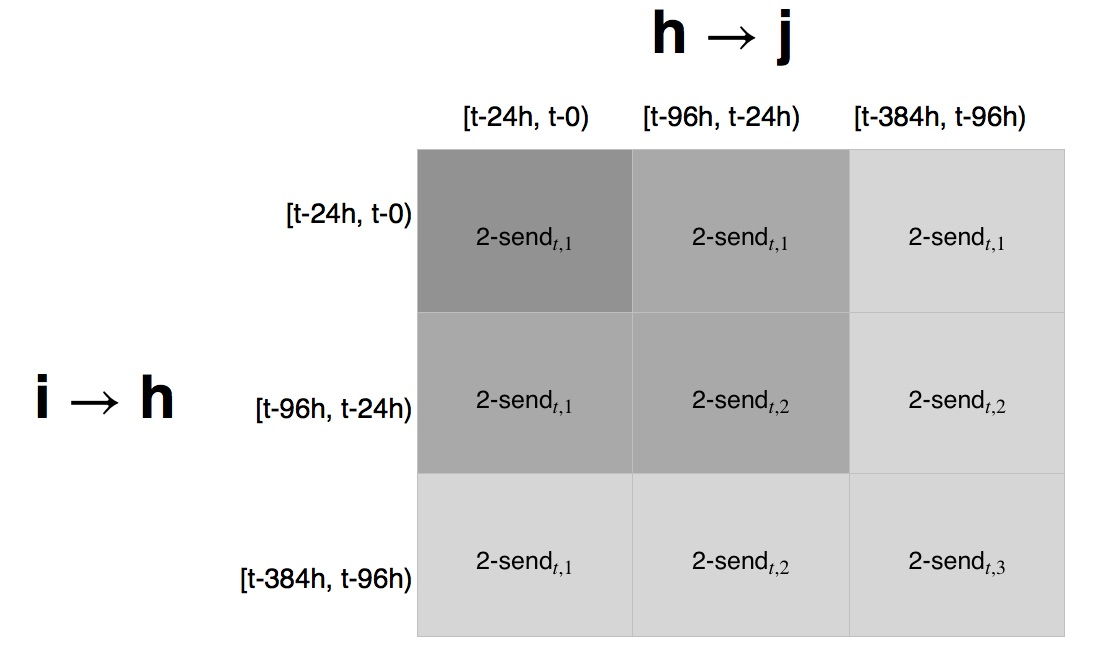
\includegraphics[width=0.76\textwidth]{triadtable.jpg} 
 	\label{fig:sim1diag}
 	\caption{Example of 2-send statistic defined for each interval $l=1,...,3$. Cells with same shades sum up to one statistic, based on when the triads are ``closed".}
 \end{figure}
In this setting, the dimension of  $\boldsymbol{b}^{(c)}$ becomes $P =  1 + 8 \times 3= 25$ for each interaction pattern $c=1,...,C$ and the corresponding $\boldsymbol{x}^{(c)}_{t}(i, j)$ consists of:
\begin{verbatim}
"intercept"    
"outdegree1"   "outdegree2"   "outdegree3"   "indegree1"    "indegree2"    "indegree3"   
"send1"        "send2"        "send3"        "receive1"     "receive2"     "receive3"     
"2-send1"      "2-send2"      "2-send3"      "2-receive1"   "2-receive2"   "2-receive3"  
"sibling1"     "sibling2"     "sibling3"     "cosibling1"   "cosibling2"   "cosibling3"   
\end{verbatim}
\subsection{Joint Generative Process of Document} \label{subsec: Joint Generative Process of Document}
 Below are the joint generative process for each document in a corpus $D$, integrating \ref{subsec: Content Generating Process}, \ref{subsec: Stochastic Intensity}, \ref{subsec: Tie Generating Process}, and \ref{subsec: Dynamic covariates2}.  
\begin{algorithm}[H]
	\SetAlgoLined
	\caption{Topic Word Distributions}
	\For{k=1 to K}{
		draw $\boldsymbol{\phi}^{(k)}$ $\sim$ Dirichlet($\beta, \bf u$)
	}
\end{algorithm}
\begin{algorithm}[H]
	\SetAlgoLined
	\caption{Interaction Pattern Parameters}
	\For{c=1 to C}{
		draw $\boldsymbol{b}^{(c)}\sim \mbox{Multivariate Normal}(\mu_{\boldsymbol{b}}, \Sigma_{\boldsymbol{b}})$
	}
\end{algorithm}
\begin{algorithm}[H]
	\SetAlgoLined
	\caption{Topic Interaction Pattern Assginments}
	\For{k=1 to K}{
		draw $C_k$ $\sim$ Uniform(1, C)
	}
\end{algorithm}
\begin{algorithm}[H]
	\SetAlgoLined
	\caption{Recipient Size Parameter}
		draw $\delta$ $\sim$ Normal($\mu_\delta, \sigma^2_\delta)$
\end{algorithm}
	\begin{algorithm}[H]
		\SetAlgoLined
		\caption{Document Generating Process}
		\For{d=1 to D}{
			draw $\bar N^{(d)}= \mbox{max}(1, N^{(d)})$\\
			draw $\boldsymbol{\theta}^{(d)}\sim \mbox{Dir}(\alpha, \boldsymbol{m})$\\
				\For{n=1 to $\bar{N}^{(d)}$}{
					draw $z_n^{(d)} \sim \mbox{Multinomial}(\boldsymbol{\theta}^{(d)})$\\
					\If {$N^{(d)}>0$} {
							draw $w_n^{(d)} \sim\mbox{Multinomial} (\boldsymbol{\phi}^{(z_n^{(d)})})$
				}
			}
                   \For{c=1 to $C$}{
                   set $p_c^{(d)} = \frac{\sum\limits_{k: c_k=c} N^{(k|d)}}{N^{(d)}}$
                   }

                    \For{i=1 to $A$}{
                    	\For{j=1 to $A$}{
                    		\If {j $\neq$ i} {
                    			  calculate $\boldsymbol{x}_{t_+^{(d-1)}}^{(c)}(i, j)$, the network statisitcs evaluated at time $t_+^{(d-1)}$  \\
                    			  set $\lambda^{(d)}_{ij}=\sum\limits_{c=1}^{C} p^{(d)}_c\cdot\mbox{exp}\Big\{\lambda_0^{(c)}+\boldsymbol{b}^{(c)T}\boldsymbol{x}^{(c)}_{t^{(d-1)}_+}(i, j)\Big\}$\\
                  }  }
                    draw $J_i^{(d)} \sim \mbox{Gibbs measure}(\{\lambda_{ij}^{(d)}\}_{j=1}^A,\delta)$\\
					draw $\Delta T_{iJ_i} \sim \mbox{Exp}(\lambda_{iJ_i}^{(d)})$
                    }
                    set $t^{(d)} = t^{(d-1)}+\mbox{min}(\Delta T_{i{J_i}})$, $i^{(d)} = i_{\mbox{min}(\Delta T_{i{J_i}})}$, and $J^{(d)} = J_{i^{(d)}}$
	}
	\end{algorithm}
	\section{Inference} \label{sec: Inference}
	  The joint generative process implies a particular factorization of the joint distribution over the variables $\Phi=\{\boldsymbol{\phi}^{(k)}\}_{k=1}^{K}, \Theta=\{\boldsymbol{\theta}^{(d)} \}_{d=1}^{D},\mathcal{Z}=\{\boldsymbol{z}^{(d)} \}_{d=1}^{D},  \mathcal{W}=\{\boldsymbol{w}^{(d)} \}_{d=1}^{D}, \mathcal{C}=\{{c}_k \}_{k=1}^{K}, \mathcal{B}=\{\boldsymbol{b}^{(c)} \}_{c=1}^{C}, \delta, \mathcal{J}=\{\{J^{(d)}_i\}_{i=1}^{A}\}_{d=1}^D,\mathcal{T}=\{  \{t_{iJ_i}^{(d)}\}_{i=1}^{A}\}_{d=1}^D$, and $\mathcal{P}=\{(i, J, t)^{(d)}\}_{d=1}^D$ given the observed $\mathcal{P}^{\prime}=\{\{(i, J, t)^{(d^\prime)}\}_{d^\prime=1}^d\}_{d=1}^D$ and the hyperparameters $(\beta, \boldsymbol{u}, \alpha, \boldsymbol{m}, \mu_{\boldsymbol{b}}, \Sigma_{\boldsymbol{b}}, \mu_\delta, \sigma^2_\delta)$:
	  \begin{equation}
	  \begin{aligned}
	  &P(\Phi, \Theta, \mathcal{Z}, \mathcal{W}, \mathcal{C}, \mathcal{B},\delta, \mathcal{J}, \mathcal{T}, \mathcal{P}|\mathcal{P}^{\prime}, \beta, \boldsymbol{u}, \alpha, \boldsymbol{m},\mu_{\boldsymbol{b}}, \Sigma_{\boldsymbol{b}}, \mu_\delta, \sigma^2_\delta) \\& 
	  = P(\Phi|\beta, \boldsymbol{u})P(\Theta|\alpha, \boldsymbol{m})P(\mathcal{Z}|\Theta)P(\mathcal{W}|\mathcal{Z}, \Phi) P(\mathcal{C})P(\mathcal{B}|\mathcal{C}, \mu_{\boldsymbol{b}}, \Sigma_{\boldsymbol{b}})P(\delta | \mu_\delta, \sigma^2_\delta)\\&\quad \quad \times
	  P(\mathcal{J}| \mathcal{Z}, \mathcal{C}, \mathcal{B}, \delta, \mathcal{P}^{\prime}, \delta)P(\mathcal{T}|\mathcal{Z}, \mathcal{C}, \mathcal{B}, \mathcal{J},  \mathcal{P}^{\prime})P(\mathcal{P}|\mathcal{J},\mathcal{T}, \mathcal{P}^{\prime}).
	  \end{aligned}
	  \end{equation}
	  We can simplify this further by integreting out $\Phi$ and $\Theta$ using Dirichlet-multinomial conjugacy (see APPENDIX \ref{subsec: phitheta integration}):
	  \begin{equation}
	  \begin{aligned}
	  &P(\mathcal{Z}, \mathcal{W}, \mathcal{C}, \mathcal{B},\delta, \mathcal{J}, \mathcal{T}, \mathcal{P}|\mathcal{P}^{\prime}, \beta, \boldsymbol{u}, \alpha, \boldsymbol{m}, \mu_{\boldsymbol{b}}, \Sigma_{\boldsymbol{b}}, \mu_\delta, \sigma^2_\delta) \\& 
	  = P(\mathcal{Z}|\alpha, \boldsymbol{m})P(\mathcal{W}|\mathcal{Z}, \beta, \boldsymbol{u} ) P(\mathcal{C})P(\mathcal{B}|\mathcal{C}, \mu_{\boldsymbol{b}}, \Sigma_{\boldsymbol{b}})P(\delta | \mu_\delta, \sigma^2_\delta) P(\mathcal{J}| \mathcal{Z}, \mathcal{C}, \mathcal{B}, \mathcal{P}^{\prime}, \delta)P(\mathcal{T}|\mathcal{Z}, \mathcal{C}, \mathcal{B}, \mathcal{J},\mathcal{P}^{\prime})P(\mathcal{P}|\mathcal{J}, \mathcal{T}, \mathcal{P}^{\prime}).
	  \end{aligned}
	  \end{equation}
	  Note that since $p_c^{(d)}$ is a deterministic function of $(\mathcal{Z}, \mathcal{C})$, $\boldsymbol{x}_{t_+^{(d-1)}}^{(c)}$ is a deterministic function of $(p_c^{(d)}, \mathcal{P}^{\prime})$  and $\boldsymbol{\lambda}^{(d)}$ is a deterministic function of $(p_c^{(d)}, \boldsymbol{x}_{t_+^{(d-1)}}^{(c)}, \mathcal{B})$, we do not include them as variables in the joint distribution. Given that $\boldsymbol{\lambda}^{(d)}$ is a function of the three latent variables $\mathcal{Z}, \mathcal{C}$, and $\mathcal{B}$, we use any parts of joint distribution that involves the term $\boldsymbol{\lambda}^{(d)}$ to make inference on $(\mathcal{Z}, \mathcal{C}, \mathcal{B})$.\\ 
	  
	 What we observe in the data is $\mathcal{W}$ and $\mathcal{P}$. We want to infer the values of all the latent variables ($\mathcal{Z}, \mathcal{C}, \mathcal{B}$) that most likely would have generated the data we observe, if we believe the generative process. Currently the variables ($\mathcal{J}, \mathcal{T}, \mathcal{P}, \mathcal{P^\prime}$) are redundant, thus we re-define the variables considering the data augmentation:   $\mathcal{J}_{\mbox{a}}=\{\{J_i^{(d)}\}_{i\neq i_o^{(d)}}\}_{d=1}^D$, and $\mathcal{T}_{\mbox{a}}=\{\{t_{iJ_i}^{(d)}\}_{i\neq i_o^{(d)}}\}_{d=1}^D$ of the augmented data and $\mathcal{I}_{\mbox{o}}=\{i_o^{(d)}\}_{d=1}^D$,  $\mathcal{J}_{\mbox{o}}=\{J_o^{(d)}\}_{d=1}^D$, and $\mathcal{T}_{\mbox{o}}= \{t^{(d)}\}_{d=1}^D$ from the observed data.\\ \newline
	  Now, our inference goal is to draw samples from the posterior distribution
	  \begin{equation}
	  \begin{aligned}
	  &P(\mathcal{Z}, \mathcal{C}, \mathcal{B}, \delta, \mathcal{J}_{\mbox{a}}, \mathcal{T}_{\mbox{a}}|\mathcal{W}, \mathcal{I}_{\mbox{o}}, \mathcal{J}_{\mbox{o}}, \mathcal{T}_{\mbox{o}}, \beta, \boldsymbol{u}, \alpha, \boldsymbol{m}, \mu_{\boldsymbol{b}}, \Sigma_{\boldsymbol{b}}, \mu_\delta, \sigma^2_\delta) \\
	  &\propto 	P(\mathcal{Z}, \mathcal{C}, \mathcal{B}, \delta, \mathcal{W}, \mathcal{J}_{\mbox{a}}, \mathcal{T}_{\mbox{a}},\mathcal{I}_{\mbox{o}}, \mathcal{J}_{\mbox{o}}, \mathcal{T}_{\mbox{o}} |\beta, \boldsymbol{u}, \alpha, \boldsymbol{m}, \mu_{\boldsymbol{b}}, \Sigma_{\boldsymbol{b}}, \mu_\delta, \sigma^2_\delta)\\&  = P(\mathcal{Z}|\alpha, \boldsymbol{m})P(\mathcal{C})P(\mathcal{B}|\mathcal{C}, \mu_{\boldsymbol{b}}, \Sigma_{\boldsymbol{b}})P(\delta | \mu_\delta, \sigma^2_\delta) P(\mathcal{W}|\mathcal{Z}, \beta, \boldsymbol{u})P(\mathcal{J}_{\mbox{a}}, \mathcal{T}_{\mbox{a}},\mathcal{I}_{\mbox{o}}, \mathcal{J}_{\mbox{o}}, \mathcal{T}_{\mbox{o}} |\mathcal{Z}, \mathcal{C}, \mathcal{B}, \delta)
	  \end{aligned}
	  \end{equation}
  As mentioned earlier in Section \ref{subsec: Tie Generating Process}, we use data augmentation in the tie generating process. Since we should include both the observed and augmented data to make inferences on the related latent variables, the derivation steps for the contribution of tie is not as smiple as other variables. Therefore, here we provide the detailed derivation steps for the last term of conditional probability: 
 \begin{equation}
\begin{aligned}
&P(\mathcal{J}_{\mbox{a}}, \mathcal{T}_{\mbox{a}},\mathcal{I}_{\mbox{o}}, \mathcal{J}_{\mbox{o}}, \mathcal{T}_{\mbox{o}} |\mathcal{Z}, \mathcal{C}, \mathcal{B}, \delta)
\\& = \prod_{d=1}^D P(\mathcal{J}^{(d)}_{\mbox{a}}, \mathcal{T}^{(d)}_{\mbox{a}}, i^{(d)}_{\mbox{o}}, J^{(d)}_{\mbox{o}}, t^{(d)}_{\mbox{o}} |\mathcal{I}^{(-d)}_{\mbox{o}}, \mathcal{J}^{(-d)}_{\mbox{o}}, \mathcal{T}^{(-d)}_{\mbox{o}},\mathcal{Z}, \mathcal{C}, \mathcal{B}, \delta)
\\& = \prod_{d=1}^D P(\mathcal{J}^{(d)}_{\mbox{a}}, \mathcal{T}^{(d)}_{\mbox{a}}, i^{(d)}_{\mbox{o}}, J^{(d)}_{\mbox{o}}, t^{(d)}_{\mbox{o}} |\mathcal{I}^{(<d)}_{\mbox{o}}, \mathcal{J}^{(<d)}_{\mbox{o}}, \mathcal{T}^{(<d)}_{\mbox{o}},\mathcal{Z}, \mathcal{C}, \mathcal{B}, \delta).
\end{aligned}
 \end{equation}
 Note that the conditional probability only depends on the past documents $(\mathcal{I}^{(<d)}_{\mbox{o}}, \mathcal{J}^{(<d)}_{\mbox{o}}, \mathcal{T}^{(<d)}_{\mbox{o}})$, but not on the future ones $(\mathcal{I}^{(>d)}_{\mbox{o}}, \mathcal{J}^{(>d)}_{\mbox{o}}, \mathcal{T}^{(>d)}_{\mbox{o}})$, since the network covariates $\boldsymbol{x}_t^{(c)}$ is calculated only based on the past interaction history. \\ \newline
Now we tackle the problem by deriving $P(\mathcal{J}^{(d)}_{\mbox{a}}, \mathcal{T}^{(d)}_{\mbox{a}}, i^{(d)}_{\mbox{o}}, J^{(d)}_{\mbox{o}}, t^{(d)}_{\mbox{o}} |\mathcal{I}^{(<d)}_{\mbox{o}}, \mathcal{J}^{(<d)}_{\mbox{o}}, \mathcal{T}^{(<d)}_{\mbox{o}}, \mathcal{Z}, \mathcal{C}, \mathcal{B}, \delta)$ for $d^{th}$ document. There are three steps involved. First is the generation of the latent receivers $J_i$ for each $i$, which corresponds to the Bernoulli part of tie generation, Equation (4); second is the generation of the observed time increment $\Delta T^{(d)} = t^{(d)} - t^{(d-1)}$ from the observed sender-receiver pairs ($i^{(d)}_{\mbox{o}}, J^{(d)}_{\mbox{o}}$), which corresponds to the Exponential tie generation in Equation (6); and the last part is the simultaneous selection process of the observed sender, receivers, and timestamp in Equation (7), implying that the latent time increments generated from the latent sender-receiver pairs were greater than the observed time increment. Reflecting the three steps, the joint distribution is:\\
 \begin{equation}
 	\begin{aligned}
 		&P(\mathcal{J}^{(d)}_{\mbox{a}}, \mathcal{T}^{(d)}_{\mbox{a}}, i^{(d)}_{\mbox{o}}, J^{(d)}_{\mbox{o}}, t^{(d)}_{\mbox{o}} |\mathcal{I}^{(<d)}_{\mbox{o}}, \mathcal{J}^{(<d)}_{\mbox{o}}, \mathcal{T}^{(<d)}_{\mbox{o}}, \mathcal{Z}, \mathcal{C}, \mathcal{B}, \delta)\\&=P\Big(\mbox{latent receivers generation}\Big) \times P\Big(\mbox{latent time generation}\Big)\times P\Big(\mbox{choose the observed}\Big) \\&
 		=\prod_{i\in \mathcal{A}}\Big(J_{i}^{(d)}\sim \mbox{Gibbs measure}(\{\lambda_{ij}^{(d)}\}_{j=1}^A,\delta)\Big) \times \prod_{i\in \mathcal{A}}\Big(\Delta T^{(d)}_{iJ_i}\sim\mbox{Exp}(\lambda^{(d)}_{iJ_i})\Big) \times \prod_{i\in \mathcal{A}_{\backslash i_o^{(d)}}} P\Big(\Delta T^{(d)}_{i{J_i}} > \Delta T_{i_{o}^{(d)}{J_{o}^{(d)}}}\Big)\\&
 		=\Big(\prod_{i\in \mathcal{A}}\frac{1}{Z(\delta,\mbox{log}(\lambda_i^{(d)}))} \exp\Big\{ \mbox{log}\big(\text{I}( \sum_{j \in \mathcal{A}_{\backslash i}} J^{(d)}_{ij} > 0 )\big) + \sum_{j \in \mathcal{A}_{\backslash i}} (\delta+\mbox{log}(\lambda_{ij}^{(d)}))J_{ij}^{(d)} \Big\}\Big)\\&\quad\quad\quad\quad\quad\quad\quad\quad\quad\quad\quad\quad\quad\quad\quad\quad\quad\quad\times \Big(\prod_{i \in\mathcal{A}}\lambda^{(d)}_{iJ_i}e^{-\Delta T^{(d)}_{iJ_i}\lambda^{(d)}_{iJ_i}}\Big)\times \Big( \prod_{i\in \mathcal{A}_{\backslash i_o^{(d)}}} e^{-\Delta T^{(d)}_{i_o^{(d)}J_o^{(d)}}\lambda^{(d)}_{iJ^{(d)}_{i}}}\Big)
 		\\&
 	\propto \Big(\prod_{i\in \mathcal{A}}\frac{1}{\Big(\prod_{j \in \mathcal{A}_{\backslash i}} \Big(\mbox{exp}\{\delta+\mbox{log}(\lambda_{ij}^{(d)})\} + 1\Big)\Big)-1}\exp\Big\{ \sum_{j \in \mathcal{A}_{\backslash i}} (\delta+\mbox{log}(\lambda_{ij}^{(d)}))J_{ij}^{(d)} \Big\}\Big)\\&\quad\quad\quad\quad\quad\quad\quad\quad\quad\quad\quad\quad\quad\quad\quad\quad\quad\quad\times\Big(\lambda^{(d)}_{i_o^{(d)}J_o^{(d)}}e^{-\Delta T^{(d)}_{i_o^{(d)}J_o^{(d)}}\lambda^{(d)}_{i_o^{(d)}J_o^{(d)}}}\Big)	\times \Big( \prod_{i\in \mathcal{A}_{\backslash i_o^{(d)}}} \lambda^{(d)}_{iJ_i}e^{-(\Delta T^{(d)}_{iJ_i} + \Delta T^{(d)}_{i_o^{(d)}J_o^{(d)}})\lambda^{(d)}_{iJ_i}}\Big),
 	\end{aligned}
 \end{equation}
We can simplify this further by integreting out the latent time $\mathcal{T}^{(d)}_{\mbox{a}}=\{\Delta T^{(d)}_{iJ_i}\}_{i \in \mathcal{A}_{\backslash i_o^{(d)}}}$ in the last term:
\begin{equation}
\begin{aligned}
&\int_{0}^\infty\cdots\int_{0}^\infty \Big(\prod_{i\in \mathcal{A}_{\backslash i_o^{(d)}}} \lambda^{(d)}_{iJ_i}e^{-(\Delta T^{(d)}_{iJ_i} + \Delta T^{(d)}_{i_o^{(d)}J_o^{(d)}})\lambda^{(d)}_{iJ_i}} \Big)d\Delta T^{(d)}_{1J_1}\cdots d\Delta T^{(d)}_{AJ_A}\\&
= \prod_{i\in \mathcal{A}_{\backslash i_o^{(d)}}} e^{- \Delta T^{(d)}_{i_o^{(d)}J_o^{(d)}}\lambda^{(d)}_{iJ_i}} \Big(\int_{0}^\infty \lambda^{(d)}_{iJ_i}e^{-\Delta T^{(d)}_{iJ_i} \lambda^{(d)}_{iJ_i}}  d\Delta T^{(d)}_{iJ_i}\Big)
\\& =\prod_{i\in \mathcal{A}_{\backslash i_o^{(d)}}} e^{- \Delta T^{(d)}_{i_o^{(d)}J_o^{(d)}}\lambda^{(d)}_{iJ_i}} \Big(\Big [ - e^{-\Delta T^{(d)}_{iJ_i} \lambda^{(d)}_{iJ_i}}\Big]_{\Delta T^{(d)}_{iJ_i}  = 0} ^{\infty}\Big)
\\& = e^{- \Delta T^{(d)}_{i_o^{(d)}J_o^{(d)}}\sum_{i\in \mathcal{A}_{\backslash i_o^{(d)}}}\lambda^{(d)}_{iJ_i}},
\end{aligned}
\end{equation}
where $\Delta T^{(d)}_{i_o^{(d)}J_o^{(d)}}$ is the observed time difference between $d^{th}$ and $(d-1)^{th}$ document.
Therefore, we can simplify Equation (12) as below:
  \begin{equation}
  \begin{aligned}
  &P(\mathcal{J}^{(d)}_{\mbox{a}}, i^{(d)}_{\mbox{o}}, J^{(d)}_{\mbox{o}}, t^{(d)}_{\mbox{o}} |\mathcal{I}^{(<d)}_{\mbox{o}}, \mathcal{J}^{(<d)}_{\mbox{o}}, \mathcal{T}^{(<d)}_{\mbox{o}}, \mathcal{Z}, \mathcal{C}, \mathcal{B}, \delta)\\&\propto \Big(\prod_{i\in \mathcal{A}}\frac{1}{\Big(\prod_{j \in \mathcal{A}_{\backslash i}} \Big(\mbox{exp}\{\delta+\mbox{log}(\lambda_{ij}^{(d)})\} + 1\Big)\Big)-1}\exp\Big\{ \sum_{j \in \mathcal{A}_{\backslash i}} (\delta+\mbox{log}(\lambda_{ij}^{(d)}))J_{ij}^{(d)} \Big\}\Big)\\&\quad\quad\quad\quad\quad\quad\quad\quad\quad\quad\quad\quad\quad\quad\quad\quad\quad\quad\times \Big(\lambda^{(d)}_{i_o^{(d)}J_{o}^{(d)}}\Big)\times\Big( e^{-\Delta T^{(d)}_{i_o^{(d)}J_o^{(d)}}\sum\limits_{i\in \mathcal{A}}\lambda^{(d)}_{iJ^{(d)}_{i}}}\Big),
  \end{aligned}
  \end{equation}
where this joint distribution can be interpreted as 'probability of latent and observed edges from non-empty Gibbs measure $\times$ probability of the observed time comes from Exponential distribution $\times$ probability of all latent time greater than the observed time, given that the latent time also come from Exponential distribution.'
Finally for implementation, we need to compute these equations in log space to prevent underflow:
 \begin{equation}
 \begin{aligned}
 &\mbox{log}\Big(P(\mathcal{J}^{(d)}_{\mbox{a}}, i^{(d)}_{\mbox{o}}, J^{(d)}_{\mbox{o}}, t^{(d)}_{\mbox{o}} |\mathcal{I}^{(<d)}_{\mbox{o}}, \mathcal{J}^{(<d)}_{\mbox{o}}, \mathcal{T}^{(<d)}_{\mbox{o}}, \mathcal{Z}, \mathcal{C}, \mathcal{B},  \delta)\Big)\\&\propto \Big(\sum_{i\in \mathcal{A}}\Big(-\log\Big(\Big(\prod_{j \in \mathcal{A}_{\backslash i}} \Big(\mbox{exp}\{\delta+\mbox{log}(\lambda_{ij}^{(d)})\} + 1\Big)\Big)-1\Big) + \sum_{j \in \mathcal{A}_{\backslash i}} (\delta+\mbox{log}(\lambda_{ij}^{(d)}))J_{ij}^{(d)}\Big)\Big)\\&\quad\quad\quad\quad\quad\quad\quad\quad\quad\quad\quad\quad\quad\quad\quad\quad\quad\quad +  \Big(\mbox{log}(\lambda^{(d)}_{i_o^{(d)}J_o^{(d)}})\Big){ - \Big(\Delta T^{(d)}_{i_o^{(d)}J_o^{(d)}}\sum\limits_{i \in \mathcal{A}}\lambda^{(d)}_{i{J_i^{(d)}}}}\Big),
 \end{aligned}
 \end{equation}
 and sequentially resample the values of each of our latent variables from their posterior distribution, conditional on all of our other variables.
    \subsection{Resampling $\mathcal{J}_{\mbox{a}}$} \label{subsec: Data augmentation}
      First of all, for each document $d$, we update the latent sender-receiver(s) pairs. That is, given the observed sender of the document $i_o^{(d)}$, we sample the latent receivers for each sender $i \in \mathcal{A}_{\backslash i_o^{(d)}}$. Here we illustrate how each sender-receiver pair in the document $d$ is updated.\\\newline
       Define ${\mathcal{J}}^{(d)}_{i}$ be the $(A-1)$ length random vector of indicators with its realization being $J^{(d)}_{i}$, representing the latent receivers corresponding to the sender $i$ in the document $d$. For each latnet sender $i$, we are going to resample ${J}^{(d)}_{ij}$, which is the $j^{th}$ element of the receiver vector ${J}^{(d)}_{i}$, one at a time with random order. The full conditional probability of ${J}^{(d)}_{ij}$ is:
       \begin{equation}
       \begin{aligned}
      & P(\mathcal{J}^{(d)}_{ij} = {J}^{(d)}_{ij}|\mathcal{J}^{(d)}_{i\backslash j}, \mathcal{Z}, \mathcal{C},   \mathcal{B}, \delta, \mathcal{W},  \mathcal{J}_{\mbox{a}, -i}, \mathcal{I}_{\mbox{o}}, \mathcal{J}_{\mbox{o}}, \mathcal{T}_{\mbox{o}}, \beta, \boldsymbol{u}, \alpha, \boldsymbol{m},  \mu_{\boldsymbol{b}}, \Sigma_{\boldsymbol{b}}, \mu_\delta, \sigma^2_\delta),
              \end{aligned}
       \end{equation}
       which we can drop some independent terms and move to 
       \begin{equation}
       \begin{aligned}
       &P(\mathcal{J}^{(d)}_{ij} = {J}^{(d)}_{ij}|\mathcal{J}^{(d)}_{i\backslash j}, i^{(d)}_{\mbox{o}}, J^{(d)}_{\mbox{o}}, t^{(d)}_{\mbox{o}}, \mathcal{I}^{(<d)}_{\mbox{o}}, \mathcal{J}^{(<d)}_{\mbox{o}}, \mathcal{T}^{(<d)}_{\mbox{o}}, \mathcal{Z}, \mathcal{C}, \mathcal{B}, \delta)\\&\propto P(\mathcal{J}^{(d)}_{ij} ={J}^{(d)}_{ij}, \mathcal{J}^{(d)}_{i\backslash j}, i^{(d)}_{\mbox{o}}, J^{(d)}_{\mbox{o}}, t^{(d)}_{\mbox{o}}| \mathcal{I}^{(<d)}_{\mbox{o}}, \mathcal{J}^{(<d)}_{\mbox{o}}, \mathcal{T}^{(<d)}_{\mbox{o}}, \mathcal{Z}, \mathcal{C}, \mathcal{B}, \delta)
       \\&\propto\Big( \frac{1}{\Big(\prod_{j \in \mathcal{A}_{\backslash i}} \Big(\mbox{exp}\{\delta+\mbox{log}(\lambda_{ij}^{(d)})\} + 1\Big)\Big)-1}\exp\Big\{\mbox{log}\big(\text{I}( \sum_{j \in \mathcal{A}_{\backslash i}} J^{(d)}_{ij} > 0 )\big) +\sum_{j \in \mathcal{A}_{\backslash i}} (\delta+\mbox{log}(\lambda_{ij}^{(d)}))J_{ij}^{(d)} \Big\}\Big)\\&\quad\quad\quad\quad\quad\quad\quad\quad\quad\quad\quad\quad\quad\quad\quad\quad\quad\quad\quad\quad\quad\times \Big(\lambda^{(d)}_{i_o^{(d)}J_{o}^{(d)}}\Big)\times \Big(e^{-\Delta T^{(d)}_{i_o^{(d)}J_o^{(d)}}\lambda^{(d)}_{iJ^{(d)}_{i}}}\Big)
       \\& \propto \Big(\exp\Big\{\mbox{log}\big(\text{I}( \sum_{j \in \mathcal{A}_{\backslash i}} J^{(d)}_{ij} > 0 )\big) +\sum_{j \in \mathcal{A}_{\backslash i}} (\delta+\mbox{log}(\lambda_{ij}^{(d)}))J_{ij}^{(d)} \Big\}\Big)\times \Big(e^{-\Delta T^{(d)}_{i_o^{(d)}J_o^{(d)}}\lambda^{(d)}_{iJ^{(d)}_{i}}}\Big),
       \end{aligned}
       \end{equation}
       where we replace typical use of $(-d)$ to $(<d)$ on the right hand side of the conditional probability, due to the fact that $d^{(th)}$ document only depends on the past documents, not on the future ones. The last line of Equation (17) is obtained by dropping the terms that do not include $J^{(d)}_{ij}$, such as the normalizing constan of Gibbs measure. \\ \newline
       To be more specific, since ${J}^{(d)}_{ij}$ could be either 1 or 0, we divide into two cases as below:
       \begin{equation}
       \begin{aligned}
       &P(\mathcal{J}^{(d)}_{ij}=1| \mathcal{J}^{(d)}_{i\backslash j}, i^{(d)}_{\mbox{o}}, J^{(d)}_{\mbox{o}}, t^{(d)}_{\mbox{o}}, \mathcal{I}^{(<d)}_{\mbox{o}}, \mathcal{J}^{(<d)}_{\mbox{o}}, \mathcal{T}^{(<d)}_{\mbox{o}}, \mathcal{Z}, \mathcal{C}, \mathcal{B}, \delta)\\& \propto \mbox{exp}\Big(\log(1) +\sum_{j \in \mathcal{A}_{\backslash i}} ( \delta+\mbox{log}(\lambda_{ij}^{(d)}))J_{i[+j]}^{(d)} -\Delta T^{(d)}_{i_o^{(d)}J_o^{(d)}}\lambda^{(d)}_{iJ^{(d)}_{ i[+j]}}\Big)
       \\& \propto \mbox{exp}\Big(\delta+\mbox{log}(\lambda_{ij}^{(d)})-\Delta T^{(d)}_{i_o^{(d)}J_o^{(d)}}\lambda^{(d)}_{iJ^{(d)}_{ i[+j]}}\Big),
       \end{aligned}
       \end{equation}
       where $J^{(d)}_{i[+j]}$ meaning that the $j^{th}$ element of $J_{i}^{(d)}$ is fixed as 1 (thus making $\mbox{log}\big(\text{I}( \sum_{j \in \mathcal{A}_{\backslash i}} J^{(d)}_{ij} > 0 )\big) = 0$ for sure). On the other hand, 
       \begin{equation}
       \begin{aligned}
       &P(\mathcal{J}^{(d)}_{ij}=0| \mathcal{J}^{(d)}_{i\backslash j}, i^{(d)}_{\mbox{o}}, J^{(d)}_{\mbox{o}}, t^{(d)}_{\mbox{o}}, \mathcal{I}^{(<d)}_{\mbox{o}}, \mathcal{J}^{(<d)}_{\mbox{o}}, \mathcal{T}^{(<d)}_{\mbox{o}}, \mathcal{Z}, \mathcal{C}, \mathcal{B}, \delta)\\& \propto \mbox{exp}\Big(\mbox{log}\big(\text{I}( \sum_{j \in \mathcal{A}_{\backslash i}} J^{(d)}_{i[-j]} > 0 )\big) + \sum_{j \in \mathcal{A}_{\backslash i}} (\delta+\mbox{log}(\lambda_{ij}^{(d)}))J_{i[-j]}^{(d)} -\Delta T^{(d)}_{i_o^{(d)}J_o^{(d)}}\lambda^{(d)}_{iJ^{(d)}_{ i[-j]}}\Big)
       \\& \propto \mbox{exp}\Big(\mbox{log}\big(\text{I}( \sum_{j \in \mathcal{A}_{\backslash i}} J^{(d)}_{i[-j]} > 0 )\big) -\Delta T^{(d)}_{i_o^{(d)}J_o^{(d)}}\lambda^{(d)}_{iJ^{(d)}_{ i[-j]}}\Big),
       \end{aligned}
       \end{equation}
       where $J^{(d)}_{i[-j]}$ meaning similarly that the $j^{th}$ element of $J_{i}^{(d)}$ is fixed as 0. In this case, we cannot guarantee that $\text{I}( \sum_{j \in \mathcal{A}_{\backslash i}} J^{(d)}_{ij} > 0)$ is 0 or 1, so we have to leave the term. When it is zero, $\exp\{\mbox{log}\big(\text{I}( \sum_{j \in \mathcal{A}_{\backslash i}} J^{(d)}_{ij} > 0 )\big)\} = 0$, thus we will sample 1 with probability 1. From this property of non-empty Gibbs measure, we prevent from the instances where the sender has no recipients to send the document. Now we can use multinomial sampling using the two probabilities, Equation (18) and Equation (19), which is equivalent to Bernoulli sampling with probability $\frac{P(\mathcal{J}^{(d)}_{ij}=1)}{P(\mathcal{J}^{(d)}_{ij}=0)+ P(\mathcal{J}^{(d)}_{ij}=0)}$. 
     \subsection{Resampling $\mathcal{Z}$}  \label{subsec: Resampling Z}
Second, we are going to resample the topic assignments, one words in a document at a time.  The new values of $z^{(d)}_n$ are sampled using the conditional posterior probability of being topic $k$ as we derived in APPENDIX \ref{subsec: conditional probability Z}:
 \begin{equation}
 \begin{aligned} & 
 P(z^{(d)}_n=k|\mathcal{Z}_{\backslash d, n},   \mathcal{C},   \mathcal{B}, \delta, \mathcal{W},  \mathcal{J}_{\mbox{a}}, \mathcal{I}_{\mbox{o}}, \mathcal{J}_{\mbox{o}}, \mathcal{T}_{\mbox{o}}, \beta, \boldsymbol{u}, \alpha, \boldsymbol{m},  \mu_{\boldsymbol{b}}, \Sigma_{\boldsymbol{b}}, \mu_\delta, \sigma^2_\delta)\\
 & \propto P(z^{(d)}_n=k, w^{(d)}_n, \mathcal{J}^{(d)}_{\mbox{a}}, i^{(d)}_{\mbox{o}}, J^{(d)}_{\mbox{o}}, t^{(d)}_{\mbox{o}}|\mathcal{Z}_{\backslash d, n}, \mathcal{C},   \mathcal{B},\delta,\mathcal{W}_{\backslash d, n}, \mathcal{I}^{(-d)}_{\mbox{o}}, \mathcal{J}^{(-d)}_{\mbox{o}}, \mathcal{T}^{(-d)}_{\mbox{o}}, \beta, \boldsymbol{u}, \alpha, \boldsymbol{m})\\
 &\propto P(z^{(d)}_n=k|\mathcal{Z}_{\backslash d, n}, \alpha, \boldsymbol{m})P(w^{(d)}_n|z^{(d)}_n=k, \mathcal{W}_{\backslash d, n}, \mathcal{Z}_{\backslash d, n}, \beta, \boldsymbol{u} )\times P(\mathcal{J}^{(d)}_{\mbox{a}}, i^{(d)}_{\mbox{o}}, J^{(d)}_{\mbox{o}}, t^{(d)}_{\mbox{o}}| z^{(d)}_n=k, \mathcal{Z}_{\backslash d, n}, \mathcal{C}, \mathcal{B}, \delta)
 \end{aligned}
 \end{equation}
 where the subscript $``{\backslash d, n}"$ denotes the exclsuion of position $n$ in $d^{th}$ document and the subscript $``{\backslash d}"$ and $``{(-d)}"$ denotes the exclsuion of $d^{th}$ document. We know that:
 \begin{equation}
 \begin{aligned} 
 P(z^{(d)}_n=k|\mathcal{Z}_{\backslash d, n}, \alpha, \boldsymbol{m})=\frac{N^{(k|d)}_{\backslash d, n}+\alpha \boldsymbol{m}_k}{N^{(d)}-1+\alpha}
 \end{aligned}
 \end{equation}
 which is the well-known form of collapsed Gibbs sampling equation for LDA. We also know that \begin{equation}
 \begin{aligned} 
 P(w^{(d)}_n|z^{(d)}_n=k, \mathcal{W}_{\backslash d, n}, \mathcal{Z}_{\backslash d, n}, \beta, \boldsymbol{u} )=\frac{N^{(w_n^{(d)}|k)}_{\backslash d, n}+\frac{\beta}{W} }{N^{(k)}_{\backslash d, n}+\beta},
 \end{aligned}
 \end{equation}
 where $N^{(w_n^{(d)}|k)}$ is the number of tokens assigned to topic $k$ whose type is the same as that of $w_n^{(d)}$, excluding $w_n^{(d)}$ itself, and $N^{(k)}_{\backslash d, n}=\sum_{w=1}^W N_{\backslash d, n}^{(w_n^{(d)}|k)}$. Finally, we already have shown that
 \begin{equation}
 \begin{aligned}
& P(\mathcal{J}^{(d)}_{\mbox{a}}, i^{(d)}_{\mbox{o}}, J^{(d)}_{\mbox{o}}, t^{(d)}_{\mbox{o}}| z^{(d)}_n=k, \mathcal{Z}_{\backslash d, n}, \mathcal{C}, \mathcal{B}, \delta)\\&=\Big( \prod_{i\in \mathcal{A}}\frac{1}{\Big(\prod_{j \in \mathcal{A}_{\backslash i}} \Big(\mbox{exp}\{\delta+\mbox{log}(\lambda_{ij}^{(d)})\} + 1\Big)\Big)-1}\exp\Big\{\sum_{j \in \mathcal{A}_{\backslash i}} (\delta+\mbox{log}(\lambda_{ij}^{(d)}))J_{ij}^{(d)} \Big\}\Big)\times \Big(\lambda^{(d)}_{i_o^{(d)}J_{o}^{(d)}}\Big)\times \Big(e^{-\Delta T^{(d)}_{i_o^{(d)}J_o^{(d)}}\lambda^{(d)}_{iJ^{(d)}_{i}}}\Big),
 \end{aligned}
 \end{equation}
 where every part includes $\lambda_{ij}^{(d)}$ such that we cannot simplify any further.\\ 
 
 Therefore, if $N^{(d)} > 0$, then the conditional probability of $n^{th}$ word in document $d$ being topic $k$ is:
 \begin{equation}
 \begin{aligned}
  &P(z^{(d)}_n=k|\mathcal{Z}_{\backslash d, n},   \mathcal{C},   \mathcal{B}, \delta, \mathcal{W}, \mathcal{J}_{\mbox{a}}, \mathcal{I}_{\mbox{o}}, \mathcal{J}_{\mbox{o}}, \mathcal{T}_{\mbox{o}}, \beta, \boldsymbol{u}, \alpha, \boldsymbol{m},  \mu_{\boldsymbol{b}}, \Sigma_{\boldsymbol{b}}, \mu_\delta, \sigma^2_\delta)\\&\propto (N^{(k|d)}_{\backslash d, n}+\alpha \boldsymbol{m}_k)\times \frac{N^{(w_n^{(d)}|k)}_{\backslash d, n}+\frac{\beta}{W} }{N^{(k)}_{\backslash d, n}+\beta}\times \Big(\prod_{i\in \mathcal{A}} \frac{1}{\Big(\prod_{j \in \mathcal{A}_{\backslash i}} \Big(\mbox{exp}\{\delta+\mbox{log}(\lambda_{ij}^{(d)})\} + 1\Big)\Big)-1}\exp\Big\{\sum_{j \in \mathcal{A}_{\backslash i}} (\delta+\mbox{log}(\lambda_{ij}^{(d)}))J_{ij}^{(d)} \Big\}\Big)\\&\quad\quad\quad\quad\quad\quad\quad\quad\quad\quad\quad\quad\quad\quad\quad\quad\quad\quad\quad\quad\quad\quad\times \Big(\lambda^{(d)}_{i_o^{(d)}J_{o}^{(d)}}\Big)\times \Big(e^{-\Delta T^{(d)}_{i_o^{(d)}J_o^{(d)}}\lambda^{(d)}_{iJ^{(d)}_{i}}}\Big), 
 \end{aligned}
 \end{equation}
 and if $N^{(d)} = 0$, then the first term becomes $\alpha\boldsymbol{m_k}$ and disappears because it is a constant. The second term disappears since there are no tokens, thus we just have the term remaining as below.
  \begin{equation}
  \begin{aligned}
  &P(z^{(d)}_1=k|\mathcal{Z}_{\backslash d, 1}=\emptyset,   \mathcal{C},   \mathcal{B}, \delta, \mathcal{W}, \mathcal{J}_{\mbox{a}}, \mathcal{I}_{\mbox{o}}, \mathcal{J}_{\mbox{o}}, \mathcal{T}_{\mbox{o}}, \beta, \boldsymbol{u}, \alpha, \boldsymbol{m},  \mu_{\boldsymbol{b}}, \Sigma_{\boldsymbol{b}}, \mu_\delta, \sigma^2_\delta)\\&\propto\Big( \prod_{i\in \mathcal{A}}\frac{1}{\Big(\prod_{j \in \mathcal{A}_{\backslash i}} \Big(\mbox{exp}\{\delta+\mbox{log}(\lambda_{ij}^{(d)})\} + 1\Big)\Big)-1}\exp\Big\{\sum_{j \in \mathcal{A}_{\backslash i}} (\delta+\mbox{log}(\lambda_{ij}^{(d)}))J_{ij}^{(d)} \Big\}\Big)\times \Big(\lambda^{(d)}_{i_o^{(d)}J_{o}^{(d)}}\Big)\times \Big(e^{-\Delta T^{(d)}_{i_o^{(d)}J_o^{(d)}}\lambda^{(d)}_{iJ^{(d)}_{i}}}\Big).
  \end{aligned}
  \end{equation}
 \subsection{Resampling $\mathcal{C}$} \label{subsec: Resampling C}
 The next variable to resample is the topic-interaction pattern assignments, one topic at a time. We derive the posterior conditional probability for the interaction pattern $\mathcal{C}$ for $k^{th}$ topic as below:
 \begin{equation}
 \begin{aligned} & P(c_k=c|\mathcal{Z},   \mathcal{C}_{\backslash k},   \mathcal{B},\delta,\mathcal{W}, \mathcal{J}_{\mbox{a}}, \mathcal{I}_{\mbox{o}}, \mathcal{J}_{\mbox{o}}, \mathcal{T}_{\mbox{o}}, \beta, \boldsymbol{u}, \alpha, \boldsymbol{m},  \mu_{\boldsymbol{b}}, \Sigma_{\boldsymbol{b}}, \mu_\delta, \sigma^2_\delta)\\
 &\propto P(c_k=c, \mathcal{J}_{\mbox{a}}, \mathcal{I}_{\mbox{o}}, \mathcal{J}_{\mbox{o}}, \mathcal{T}_{\mbox{o}}|\mathcal{Z}, \mathcal{C}_{\backslash k},   \mathcal{B},\delta)\\
& \propto P(c_k=c)P(\mathcal{J}_{\mbox{a}}, \mathcal{I}_{\mbox{o}}, \mathcal{J}_{\mbox{o}}, \mathcal{T}_{\mbox{o}}| \mathcal{Z}, c_k=c, \mathcal{C}_{\backslash k}, \mathcal{B}, \delta)
 \end{aligned}
 \end{equation}
 where $P(c_k=c) = \frac{1}{C}$ so this term disappears. Therefore, 
 \begin{equation}
 \begin{aligned}
 &P(c_k=c|\mathcal{Z},   \mathcal{C}_{\backslash k},   \mathcal{B}, \delta, \mathcal{W}, \mathcal{I}_{\mbox{a}}, \mathcal{J}_{\mbox{a}}, \mathcal{I}_{\mbox{o}}, \mathcal{J}_{\mbox{o}}, \mathcal{T}_{\mbox{o}}, \beta, \boldsymbol{u}, \alpha, \boldsymbol{m},  \mu_{\boldsymbol{b}}, \Sigma_{\boldsymbol{b}}, \mu_\delta, \sigma^2_\delta)\\&\propto P( \mathcal{J}_{\mbox{a}}, \mathcal{I}_{\mbox{o}}, \mathcal{J}_{\mbox{o}}, \mathcal{T}_{\mbox{o}}| \mathcal{Z}, c_k=c, \mathcal{C}_{\backslash k}, \mathcal{B}, \delta)\\&=\prod_{d=1}^D\Bigg(\Big(\prod_{i\in \mathcal{A}} \frac{1}{\Big(\prod_{j \in \mathcal{A}_{\backslash i}} \Big(\mbox{exp}\{\delta+\mbox{log}(\lambda_{ij}^{(d)})\} + 1\Big)\Big)-1}\exp\Big\{\sum_{j \in \mathcal{A}_{\backslash i}} (\delta+\mbox{log}(\lambda_{ij}^{(d)}))J_{ij}^{(d)} \Big\}\Big)\\&\quad\quad\quad\quad\quad\quad\quad\quad\quad\quad\quad\quad\quad\quad\quad\quad\quad\quad\times \Big(\lambda^{(d)}_{i_o^{(d)}J_{o}^{(d)}}\Big)\times \Big(e^{-\Delta T^{(d)}_{i_o^{(d)}J_o^{(d)}}\lambda^{(d)}_{iJ^{(d)}_{i}}}\Big)\Bigg),
 \end{aligned}
 \end{equation} 
 with $c_k=c$ throughout. Note that in the product over $d$, we only need to consider those emails that actually use topic $k$; the others will have no terms involving $c_k$.
 \subsection{Resampling $\mathcal{B}$ }  \label{subsec: Resampling B}
Next, we update $\mathcal{B}=\{\boldsymbol{b}^{(c)}\}_{c=1}^C$. For this, we use the Metropolis-Hastings algorithm with a proposal density $Q$ being the multivariate Gaussian distribution, with a diagonal covariance matrix multiplied by $\sigma^2_Q$ (proposal distribution variance parameters set by the user), centered on the current values of $\mathcal{B}=\{\boldsymbol{b}^{(c)}\}_{c=1}^C$. Under the symmetric proposal distribution, we cancel out Q-ratio and then accept the new proposed value $\mathcal{B}^\prime=\{\boldsymbol{b}^{\prime(c)}\}_{c=1}^C$ with probability equal to:
 \begin{equation}
 \begin{split}
 & \mbox{Acceptance Probability}=
 \begin{cases}  \frac{P(\mathcal{B}^\prime|\mathcal{Z},   \mathcal{C}, \delta, \mathcal{W},  \mathcal{J}_{\mbox{a}}, \mathcal{I}_{\mbox{o}}, \mathcal{J}_{\mbox{o}}, \mathcal{T}_{\mbox{o}}, \beta, \boldsymbol{u}, \alpha, \boldsymbol{m},\mu_{\boldsymbol{b}}, \Sigma_{\boldsymbol{b}}, \mu_\delta, \sigma^2_\delta)}{P(\mathcal{B}|\mathcal{Z},   \mathcal{C}, \delta, \mathcal{W}, \mathcal{J}_{\mbox{a}}, \mathcal{I}_{\mbox{o}}, \mathcal{J}_{\mbox{o}}, \mathcal{T}_{\mbox{o}}, \beta, \boldsymbol{u}, \alpha, \boldsymbol{m}, \mu_{\boldsymbol{b}}, \Sigma_{\boldsymbol{b}}, \mu_\delta, \sigma^2_\delta)}\quad\text{if}  <1\\
 1 \quad \text{else}
 \end{cases}
 \end{split}
 \end{equation}
 After factorization, we get
 \begin{equation}
 \begin{aligned}
& \frac{P(\mathcal{B}^\prime|\mathcal{Z},   \mathcal{C},  \delta, \mathcal{W}, \mathcal{J}_{\mbox{a}}, \mathcal{I}_{\mbox{o}}, \mathcal{J}_{\mbox{o}}, \mathcal{T}_{\mbox{o}}, \beta, \boldsymbol{u}, \alpha, \boldsymbol{m}, \mu_{\boldsymbol{b}}, \Sigma_{\boldsymbol{b}}, \mu_\delta, \sigma^2_\delta)}{P(\mathcal{B}|\mathcal{Z},   \mathcal{C}, \delta, \mathcal{W}, \mathcal{J}_{\mbox{a}},\mathcal{I}_{\mbox{o}}, \mathcal{J}_{\mbox{o}}, \mathcal{T}_{\mbox{o}}, \beta, \boldsymbol{u}, \alpha, \boldsymbol{m}, \mu_{\boldsymbol{b}}, \Sigma_{\boldsymbol{b}}, \mu_\delta, \sigma^2_\delta)}\\=&\frac{P(\mathcal{Z}, \mathcal{C}, \mathcal{B}^\prime, \delta, \mathcal{W},  \mathcal{J}_{\mbox{a}}, \mathcal{I}_{\mbox{o}}, \mathcal{J}_{\mbox{o}}, \mathcal{T}_{\mbox{o}} |\beta, \boldsymbol{u}, \alpha, \boldsymbol{m}, \mu_{\boldsymbol{b}}, \Sigma_{\boldsymbol{b}}, \mu_\delta, \sigma^2_\delta)}{P(\mathcal{Z}, \mathcal{C}, \mathcal{B}, \delta, \mathcal{W}, \mathcal{J}_{\mbox{a}}, \mathcal{I}_{\mbox{o}}, \mathcal{J}_{\mbox{o}}, \mathcal{T}_{\mbox{o}} |\beta, \boldsymbol{u}, \alpha, \boldsymbol{m}, \mu_{\boldsymbol{b}}, \Sigma_{\boldsymbol{b}}, \mu_\delta, \sigma^2_\delta)}\\=&\frac{P(\mathcal{B}^\prime|\mathcal{C}, \mu_{\boldsymbol{b}}, \Sigma_{\boldsymbol{b}})P(\mathcal{J}_{\mbox{a}}, \mathcal{I}_{\mbox{o}}, \mathcal{J}_{\mbox{o}}, \mathcal{T}_{\mbox{o}} |\mathcal{Z}, \mathcal{C}, \mathcal{B}^\prime, \delta)}{P(\mathcal{B}|\mathcal{C}, \mu_{\boldsymbol{b}}, \Sigma_{\boldsymbol{b}})P(\mathcal{J}_{\mbox{a}}, \mathcal{I}_{\mbox{o}}, \mathcal{J}_{\mbox{o}}, \mathcal{T}_{\mbox{o}} |\mathcal{Z}, \mathcal{C}, \mathcal{B}, \delta)},
 \end{aligned}
 \end{equation}
 where $P(\mathcal{B}|\mathcal{C}, \mu_{\boldsymbol{b}}, \Sigma_{\boldsymbol{b}})$ is calculated from the product of $\boldsymbol{b}^{(c)}\sim \mbox{Multivariate Normal}(\mu_{\boldsymbol{b}}, \Sigma_{\boldsymbol{b}}$) over the interaction patterns $c \in \{1,...,C\}$ (as defined in Section \ref{sec: Generative Process}) and $P(\mathcal{J}_{\mbox{a}}, \mathcal{I}_{\mbox{o}}, \mathcal{J}_{\mbox{o}}, \mathcal{T}_{\mbox{o}} |\mathcal{Z}, \mathcal{C}, \mathcal{B}, \delta)$ is the same as Equation (27). Again, we take the log and obtain the log of acceptance ratio:
 \begin{equation}
 \begin{aligned} 
 &\sum_{c=1}^C\mbox{log}\Big(\mathcal{N}(\boldsymbol{b}^{\prime(c)};\mu_{\boldsymbol{b}}, \Sigma_{\boldsymbol{b}})\Big)-\sum_{c=1}^C\mbox{log}\Big(\mathcal{N}(\boldsymbol{b}^{(c)};\mu_{\boldsymbol{b}}, \Sigma_{\boldsymbol{b}})\Big)\\&+ \sum_{d=1}^D\Bigg(\Big(\sum_{i\in \mathcal{A}}\Big(-\log\Big(\Big(\prod_{j \in \mathcal{A}_{\backslash i}} \Big(\mbox{exp}\{\delta+\mbox{log}(\lambda_{ij}^{(d)})\} + 1\Big)\Big)-1\Big) + \sum_{j \in \mathcal{A}_{\backslash i}} (\delta+\mbox{log}(\lambda_{ij}^{(d)}))J_{ij}^{(d)}\Big)\\&\quad\quad\quad\quad\quad\quad\quad\quad\quad\quad\quad\quad\quad\quad\quad\quad\quad\quad +  \Big(\mbox{log}(\lambda^{(d)}_{i_o^{(d)}J_o^{(d)}}){ - \Delta T^{(d)}_{i_o^{(d)}J_o^{(d)}}\sum\limits_{i \in \mathcal{A}}\lambda^{(d)}_{i{J_i^{(d)}}}} \Big)\mbox{ given }  \boldsymbol{b}^\prime\Bigg)
 \\& -\sum_{d=1}^D\Bigg(\Big(\sum_{i\in \mathcal{A}}\Big(-\log\Big(\Big(\prod_{j \in \mathcal{A}_{\backslash i}} \Big(\mbox{exp}\{\delta+\mbox{log}(\lambda_{ij}^{(d)})\} + 1\Big)\Big)-1\Big) + \sum_{j \in \mathcal{A}_{\backslash i}} (\delta+\mbox{log}(\lambda_{ij}^{(d)}))J_{ij}^{(d)}\Big)\\&\quad\quad\quad\quad\quad\quad\quad\quad\quad\quad\quad\quad\quad\quad\quad\quad\quad\quad +  \Big(\mbox{log}(\lambda^{(d)}_{i_o^{(d)}J_o^{(d)}}){ - \Delta T^{(d)}_{i_o^{(d)}J_o^{(d)}}\sum\limits_{i \in \mathcal{A}}\lambda^{(d)}_{i{J_i^{(d)}}}} \Big)\mbox{ given }  \boldsymbol{b}\Bigg),
 \end{aligned}
 \end{equation}
 where $\mathcal{N}$ is the multivariate normal density. Then the log of acceptance ratio we have is:
 \begin{equation}
 \mbox{log(Acceptance Probability) = min(Equation (30), 0). }
 \end{equation}
 To determine whether to accept the proposed update or not, we use the log of acceptance ratio; if the log of a sample from Uniform(0,1) is less than the log-acceptance probability (30), we accept the proposal $\boldsymbol{b}^\prime$. Otherwise, we reject.
  \subsection{Resampling $\delta$ }  \label{subsec: Resampling delta}
Finally we move on to the updates of $\delta$, which is very similar to the steps illustrated in Section \ref{subsec: Resampling B}. Again we use Metropolis-Hastings algorithm with Normal proposal distribution such that we can cancel out the Q-ratio. We may change the proposal variance $\sigma^2_\delta$ to ensure appropriate level of acceptance rate. Then, it follows that the simplified version of acceptance probability is 
\begin{equation} 
	\begin{split}
		& \mbox{Acceptance Probability}=
		\begin{cases}  \frac{P(\delta^\prime|\mu_\delta, \sigma^2_\delta) P(\mathcal{J}_{\mbox{a}}, \mathcal{I}_{\mbox{o}}, \mathcal{J}_{\mbox{o}}, \mathcal{T}_{\mbox{o}} |\mathcal{Z}, \mathcal{C}, \mathcal{B}, \delta^\prime)}{P(\delta|\mu_\delta, \sigma^2_\delta) P(\mathcal{J}_{\mbox{a}}, \mathcal{I}_{\mbox{o}}, \mathcal{J}_{\mbox{o}}, \mathcal{T}_{\mbox{o}} |\mathcal{Z}, \mathcal{C}, \mathcal{B}, \delta)}\quad\text{if}  <1\\
			1 \quad \text{else}
		\end{cases}
	\end{split}
\end{equation}
By taking the log, we obtain the log of acceptance ratio:
\begin{equation}
	\begin{aligned} 
		&\mbox{log}\Big(\mathcal{N}(\delta^\prime;\mu_\delta, \sigma^2_\delta)\Big)-\mbox{log}\Big(\mathcal{N}(\delta; \mu_\delta, \sigma^2_\delta)\Big)\\&+ \sum_{d=1}^D\Bigg(\sum_{i\in \mathcal{A}}\Big(-\log\Big(\Big(\prod_{j \in \mathcal{A}_{\backslash i}} \Big(\mbox{exp}\{\delta^\prime+\mbox{log}(\lambda_{ij}^{(d)})\} + 1\Big)\Big)-1\Big) + \sum_{j \in \mathcal{A}_{\backslash i}} (\delta^\prime+\mbox{log}(\lambda_{ij}^{(d)}))J_{ij}^{(d)}\Big)
		\\&\quad\quad -\sum_{i\in \mathcal{A}}\Big(-\log\Big(\Big(\prod_{j \in \mathcal{A}_{\backslash i}} \Big(\mbox{exp}\{\delta+\mbox{log}(\lambda_{ij}^{(d)})\} + 1\Big)\Big)-1\Big) + \sum_{j \in \mathcal{A}_{\backslash i}} (\delta+\mbox{log}(\lambda_{ij}^{(d)}))J_{ij}^{(d)}\Big)\Bigg),
	\end{aligned}
\end{equation}
and the corresponding log of acceptance ratio is
\begin{equation}
	\mbox{log(Acceptance Probability) = min(Equation (33), 0). }
\end{equation}
 \subsection{Pseudocode}  \label{subsec: Pseudocode}
 To implement the inference procedure outlined above, we provide a pseudocode for Markov Chain Monte Carlo (MCMC) sampling. For better performance, we implement $n_1$ iteration of the hyperparameter optimization technique called ``new fixed-point iterations using the Digamma recurrence relation'' in \cite{wallach2008structured} based on Minka’s fixed-point iteration \citep{minka2000estimating}, for every outer iteration $o$. Also, while we update the categorical variables $\mathcal{Z}$ and $\mathcal{C}$ once per outer iteration, we specify larger number of inner iterations ($n_2$ and $n_3$) for the continuous variables $\mathcal{B}$ and $\delta$, which converge slowly than the discrete variables. When summarizing model results, we only use the samples from the last $O^{th}$ outer loop.
 \begin{algorithm}[H]
 	\SetAlgoLined
 	\caption{MCMC}
 	set initial values $\mathcal{Z}^{(0)}, \mathcal{C}^{(0)}, $ and $(\mathcal{B}^{(0)}, \delta^{(0)})$\\
 	\For{o=1 to O}{
 			\For{n=1 to $n_1$}{
 		optimize $\alpha$ and $\boldsymbol{m}$ using hyperparameter optimization in \cite{wallach2008structured}
 	}
 			\For{d=1 to D}{
 				\For{i $\in \mathcal{A}_{\backslash i_o^{(d)}}$}{
 				sample the augmented data $J^{(d)}_i$ following Section \ref{subsec: Data augmentation}
 			}
 					\For{n=1 to $N^{(d)}$}{
 						draw of $z_n^{(d)}\sim\mbox{Multinomial}(p^\mathcal{Z})$ following Section \ref{subsec: Resampling Z}}}
 			\For{k=1 to K}{
 				draw $C_k\sim \mbox{Multinomial}(p^\mathcal{C})$ following Section \ref{subsec: Resampling C}
 				}
	\For{n=1 to $n_2$}{
 			sample $\mathcal{B}$ using M-H following Section \ref{subsec: Resampling B}
 		}
 		\For{n=1 to $n_3$}{
 			sample $\delta$ using M-H following Section \ref{subsec: Resampling delta}
  		}
 	}	Summarize the results with:\\
 	last sample of $\mathcal{C}$, last sample of $\mathcal{Z}$, last $n_2$ length chain of $\mathcal{B}$, last $n_3$ length chain of $\delta$ 
 \end{algorithm}
   \section{Getting It Right (GiR)}
        \subsection{Collapsed-time Tie Generating Process} \label{subsubsec: collapsed time Generative Process}
        Considering that we integrated out latent time $\mathcal{T}_{\mbox{a}}$ in the inference, we develop the new generative process for (sender, recipients, timestamp) parts with latent time integrated out. Note that this is built upon the property of the minimum of independent Exponential random variables (the probability $\Delta T_{i{J_i}}$ being the minimum is $\frac{\lambda_{i{J_i}}^{(d)}}{\sum_{i=1}^A\lambda_{i{J_i}}^{(d)}}$). Details are illustrated in Algorithm 7.
        \begin{algorithm}[H]
        	\SetAlgoLined
        	\caption{Collapsed-time Tie Generating Process}
        	\For{d=1 to D}{
        		\For{i=1 to $A$}{
        			\For{j=1 to $A$}{
        				\If {j $\neq$ i} {
        					calculate $\boldsymbol{x}_{t_+^{(d-1)}}^{(c)}(i, j)$, the network statisitcs evaluated at time $t_+^{(d-1)}$  \\
        					set $\lambda^{(d)}_{ij}=\sum\limits_{c=1}^{C} p^{(d)}_c\cdot\mbox{exp}\Big\{\lambda_0^{(c)}+\boldsymbol{b}^{(c)T}\boldsymbol{x}^{(c)}_{t^{(d-1)}_+}(i, j)\Big\}\cdot 1\{j \in \mathcal{A}_{\backslash i}\}$}  
        			}
        			draw $J_i^{(d)} \sim \mbox{Gibbs measure}(\{\lambda_{ij}^{(d)}\}_{j=1}^A,\delta)$\\
        			calculate $\lambda_{i{J_i}}^{(d)}$\\
        		}
        		choose $i^{(d)} \sim {\mbox{Multinomial}(\{\frac{\lambda_{i{J_i}}^{(d)}}{\sum\limits_{i \in \mathcal{A}}\lambda_{i{J_i}}^{(d)}}\}_{i=1}^A)}$\\
        		set $J^{(d)} = J_{i^{(d)}}$\\
        		draw $\Delta T_{i^{(d)}J^{(d)}} \sim \mbox{Exponential}(\sum\limits_{i \in \mathcal{A}}\lambda_{i{J_i}}^{(d)})$ and set $t^{(d)} = t^{(d-1)} + \Delta T_{i^{(d)}J^{(d)}}$
        	}
        \end{algorithm}
        \noindent With this generative process, the joint likelihood (comparable to Equation (12)) becomes:
        \begin{equation}
        \begin{aligned}
        &P(\mathcal{J}^{(d)}_{\mbox{a}}, \mathcal{T}^{(d)}_{\mbox{a}}, i^{(d)}_{\mbox{o}}, J^{(d)}_{\mbox{o}}, t^{(d)}_{\mbox{o}} |\mathcal{I}^{(<d)}_{\mbox{o}}, \mathcal{J}^{(<d)}_{\mbox{o}}, \mathcal{T}^{(<d)}_{\mbox{o}}, \mathcal{Z}, \mathcal{C}, \mathcal{B}, \delta)\\&=P\Big(\mbox{latent receivers generation}\Big) \times P\Big(\mbox{choose the sender}\Big)\times P\Big(\mbox{observed minimum time generation}\Big) \\&
        =\prod_{i\in \mathcal{A}}\Big(J_{i}^{(d)}\sim \mbox{Gibbs measure}(\{\lambda_{ij}^{(d)}\}_{j=1}^A,\delta)\Big) \times \Big(i_o^{(d)} \sim \mbox{Multinom}(\{\frac{\lambda_{i{J_i}}^{(d)}}{\sum\limits_{i \in \mathcal{A}}\lambda_{i{J_i}}^{(d)}}\}_{i=1}^A)\Big) \times\Big(\Delta T^{(d)}_{i^{(d)}{J^{(d)}}} \sim \mbox{Exp}(\sum\limits_{i \in \mathcal{A}}\lambda_{i_o^{(d)}J_o^{(d)}}^{(d)})\Big)\\&
        =\Big(\prod_{i\in \mathcal{A}}\frac{1}{Z(\delta, \log(\lambda^{(d)}_i)}\exp\Big\{ \sum_{j \in \mathcal{A}_{\backslash i}} (\delta+\mbox{log}(\lambda_{ij}^{(d)}))J_{ij}^{(d)} \Big\}\Big)\times \Big(\frac{\lambda_{i_o^{(d)}J_o^{(d)}}^{(d)}}{\sum\limits_{i \in \mathcal{A}}\lambda_{i{J_i}}^{(d)}}\Big)\times \Big((\sum\limits_{i \in \mathcal{A}}\lambda_{i{J_i}}^{(d)})e^{-\Delta T^{(d)}_{i_o^{(d)}J_o^{(d)}}\sum\limits_{i \in \mathcal{A}}\lambda_{i{J_i}}^{(d)}}\Big)
        \\&
        =\Big(\prod_{i\in \mathcal{A}}\frac{1}{Z(\delta, \log(\lambda^{(d)}_i)}\exp\Big\{ \sum_{j \in \mathcal{A}_{\backslash i}} (\delta+\mbox{log}(\lambda_{ij}^{(d)}))J_{ij}^{(d)} \Big\}\Big)\times\Big(\frac{\lambda_{i_o^{(d)}J_o^{(d)}}^{(d)}}{\sum\limits_{i \in \mathcal{A}}\lambda_{i{J_i}}^{(d)}}\Big)\times \Big( (\sum\limits_{i \in \mathcal{A}}\lambda_{i{J_i}}^{(d)})e^{-\Delta T^{(d)}_{i_o^{(d)}J_o^{(d)}}\sum\limits_{i \in \mathcal{A}}\lambda_{i{J_i}}^{(d)}}\Big)\\& \propto \Big(\prod_{i\in \mathcal{A}}\frac{1}{\Big(\prod_{j \in \mathcal{A}_{\backslash i}} \Big(\mbox{exp}\{\delta+\mbox{log}(\lambda_{ij}^{(d)})\} + 1\Big)\Big)-1}\exp\Big\{ \sum_{j \in \mathcal{A}_{\backslash i}} (\delta+\mbox{log}(\lambda_{ij}^{(d)}))J_{ij}^{(d)} \Big\}\Big)\\&\quad\quad\quad\quad\quad\quad\quad\quad\quad\quad\quad\quad\quad\quad\quad\quad\quad\quad\quad\quad\quad\quad\quad\quad\quad\quad\times\Big(\lambda_{i_o^{(d)}J_o^{(d)}}^{(d)}\Big)\times \Big( e^{-\Delta T^{(d)}_{i_o^{(d)}J_o^{(d)}}\sum\limits_{i \in \mathcal{A}}\lambda_{i{J_i}}^{(d)}}\Big),
        \end{aligned}
        \end{equation}
        which is exactly the same as Equation (14), thus we will use this collpased-time generative process as a forward/backward generative process in Geweke’s “Getting it Right” test \citep{geweke2004getting}.
       \subsection{Backward Generating Process} \label{subsubsec: Backward Generative Process}
   We need to define a “backward” generative process in order to perform Geweke’s “Getting it Right” (GiR) test because when we are generating our “backwards” samples, we only want to resample the token word types given the token-topic assignments (using Collapsed Gibbs sampling) and (sender, recipients, timestamp) pairs, and not any of
   our latent variables. This means we take the latent variables we got by running our inference procedure (latent edges from data augmentation, token topic assignments, topic interaction pattern assignments, interaction pattern parameters, and receiver size parameter $\delta$) as inputs, and simply condition on these to draw new data. \\
   
For backward sampling, we let $NKV$ be a $V\times K$ dimensional matrix where each entry will record the count of the number of tokens of word-type $v$ that are currently assigned to topic $k$. Also let $NK$ be a $K$ dimensional vector recording the total count of tokens currently assigned to topic $k$. In addition, here we do not generate latent edges, instead, we use inferred ones from the inference as an input. Only the receivers for previously observed sender ($i_o^{(d)}$), which is not inferred, will be sampled according to the generative process, same as forward sampling (with inferred parameter values). This “backward” version of the generative process is detailed below in Algorithm 8.
   \begin{algorithm}[H]
   	\SetAlgoLined
   	\caption{Generate data with backward sampling}
   	Input:\\ 1) latent edges $\{\{iJ^{(d)}_i\}_{i \neq i_o^{(d)}}\}_{d=1}^D$ (where $\{i_o^{(d)}\}_{d=1}^D$ from previous backward sample),\\
   	 2) token topic assignments $\{\{z_n^{(d)}\}_{n=1}^{N^{(d)}}\}_{d=1}^D$,\\
   	 3) topic interaction pattern assignments, $\{C_k\}_{k=1}^K$,\\
   	   4) interaction pattern parameters $\{\boldsymbol{b}^{(c)}\}_{c=1}^C$, \\
   	   5) receiver size parameter $\delta$.\\\\
   	\For{d=1 to D}{
   		set $NKV = 0$ and $NK = 0$\\
   		\For{n=1 to $\bar {N}^{(d)}$}{
   				\For{v=1 to $V$}{
   					$\mbox{token-word-type-distribution}_n^{(d)}[v] = \frac{NKV_{v, z_n^{(d)}}+\beta\boldsymbol{u}_v}{NK_{z_n^{(d)}} + \beta}$
   				}
   				draw $w_n^{(d)} \sim (\mbox{token-word-type-distribution}_n^{(d)})$\\
   				$NKV_{w_n^{(d)}, z_n^{(d)}} += 1$\\
   				$NK_{z_n^{(d)}} += 1$
   		}
   		only for the previously observed sender $i_o^{(d)}$,\\
   				\For {j $\neq$ $i_o^{(d)}$} {
   					calculate $\boldsymbol{x}_{t_+^{(d-1)}}^{(c)}(i_o^{(d)}, j)$, the network statisitcs evaluated at time $t_+^{(d-1)}$  \\
   					set $\lambda^{(d)}_{i_o^{(d)}j}=\sum\limits_{c=1}^{C} p^{(d)}_c\cdot\mbox{exp}\Big\{\lambda_0^{(c)}+\boldsymbol{b}^{(c)T}\boldsymbol{x}^{(c)}_{t^{(d-1)}_+}(i_o^{(d)}, j)\Big\}\cdot 1\{j \in \mathcal{A}_{\backslash i_o^{(d)}}\}$\\
   					}  
   		draw $J_{i_o^{(d)}}^{(d)} \sim \mbox{Gibbs measure}(\{\lambda_{{i_o^{(d)}}j}^{(d)}\}_{j=1}^A,\delta)$\\			
   		choose $i^{(d)} \sim {\mbox{Multinomial}(\{\frac{\lambda_{i{J_i}}^{(d)}}{\sum\limits_{i \in \mathcal{A}}\lambda_{i{J_i}}^{(d)}}\}_{i=1}^A)}$ \\
   		set $J^{(d)} = J_{i^{(d)}}$\\
   		draw $\Delta T_{i^{(d)}J^{(d)}} \sim \mbox{Exponential}(\sum\limits_{i \in \mathcal{A}}\lambda_{i{J_i}}^{(d)})$ and set $t^{(d)} = t^{(d-1)} + \Delta T_{i^{(d)}J^{(d)}}$
   	}
   \end{algorithm}
      \subsection{Intitialization of History $\boldsymbol{x}_t^{(c)}$} \label{subsubsec: Initial history issue}
      Considering that our network statistics $\boldsymbol{x}_t^{(c)}$ are generated by the network itself, it is necessary to use the same initial value of $\boldsymbol{x}_t^{(c)}$ across the forward and backward samples. If not, when we generate fixed number of documents (e.g. nDocs = 10), we cannot guarantee the same number of documents used for the inference, since only the documents with its timestamp greater than 384 hours (=16 days) are used in the inference. In the extreme cases, we may end up with two types of failure:
      \begin{itemize}
      	\item[1.] Zero document generated after 384 hours (i.e. $t^{(10)} < 384$), making no documents to be used for inference,
      	\item[2.] Zero document generated before 384 hours (i.e. $t^{(1)} > 384$), making the estimate of $\mathcal{B}$ totally biased since $\forall  \boldsymbol{x}_t^{(c)}(i, j) = 0$. 
      \end{itemize}
      Therefore, we fix the initial state of $\boldsymbol{x}_t^{(c)}$ over the entire GiR process. Specifically, we fix 30 (for example) baseline documents where the timestamps are all smaller than 384 and use as an input for forward sampling, backward sampling, and the inference. Then, in the forward and backward generative process, we set the starting point of the timestamp as $t^{(0)} = 384$ and generate nDocs = 10 documents given the initial $\boldsymbol{x}_{t^{(0)} = 384}^{(c)}$ so that we can acheive consistency in the generated number of documents with $t^{(d)} > 384$.
   \subsection{GiR Implementation Details} \label{subsubsec: GiR implementation}
   While we tried a number of different parameter combinations in the course of testing, we outline our standard setup. We selected the following parameter values:
   \begin{itemize}
   	\begin{minipage}{0.5\textwidth}
   		\item[-] nDocs (number of documents) = 5
   		\item[-] nwords (tokens per document) = 4
   		\item[-] node (number of actors)= 4
   		\item[-] W (unique word types) = 5
   		\item[-] nIP (number of interaction patterns) = 2
   		\item[-] K (number of topics) = 4
   		\item[-] $\alpha$ (Dirichlet concentration prior) = 2
   		\item[-] $\boldsymbol{m}$ (Dirichlet base prior) = $\boldsymbol{u}$ 
   		\item[-] $\beta$ (Dirichlet concentration prior)= 2
   		\item[-] $\boldsymbol{n}$ (Dirichlet base prior) = $\boldsymbol{u}$
   		\item[-] netstat = ``intercept" and ``dyadic"
   	\end{minipage}
   	\begin{minipage}{0.5\textwidth}
   		\item[-] prior for $\boldsymbol{b}^{(c)}$: $\mu_{\boldsymbol{b}^{(c)}} = (-3,\boldsymbol{0}_6), \Sigma_{\boldsymbol{b}^{(c)}} = 0.005\times I_7$
   		\item[-] prior for $\delta$: $\mu_\delta = 0$, $\sigma^2_\delta = 0.1$
   		\item[-] $I$ (outer iteration) = 3
   		\item[-] $n_1$ (iteration for hyperparamter optimization) = 0
   		\item[-] $n_2$ (M-H sampling iteration of $\mathcal{B}$) = 330
   		\item[-] burn (M-H sampling burn-in of $\mathcal{B}$)= 30
   		\item[-] thin (M-H sampling thinning of $\mathcal{B}$)= 3
   		\item[-] $\sigma_{Q1}^2$ (proposal variance for $\mathcal{B}$) = 0.04
   		\item[-] $n_3$ (M-H sampling iteration of $\delta$) = 10
   		\item[-] $\sigma_{Q2}^2$ (proposal variance for $\delta$) = 2
   	\end{minipage}
   \end{itemize}
   Next, we list the selection of statistics we save for each forward and backward sample. Note that these statistics are not sensitive to the label swithches across the updates. Therefore, at each iteration, we calculate and save the statistics below:
      \begin{itemize}
      	\item[1.] Mean of interaction pattern parameters $(\boldsymbol{b}_p^{(1)},...,\boldsymbol{b}_p^{(C)})$ for every $p = 1,...,P$,
      	      	\item[2.] Three istory statistic `send' calculated for the last document
      	      	\item[3.] $\delta$ value used to generate the samples
      	      	\item[4.] Mean number of recipients,
      	\item[5.] Mean of time-increments $t^{(d)}-t^{(d-1)}$ for every $d=2,...,\mbox{nDocs}$,
      	\item[6.] Mean topic-interaction pattern assignment (for interaction patterns indexed by 1 and 2), 
      	\item[7.] Number of tokens in topics assigned to each interaction pattern $c=1,...,C$,
      	\item[8.] Number of tokens assigned to each topic $k=1,...,K$, 
       \item[9.] Number of tokens assigned to each unique word type $w=1,...,W$.
      	      \end{itemize}
\subsection{GiR Results}
Having saved a set of samples, we generated PP (Probability-Probability)  plots for each of the 25 statistics we saved. We calculated 1,000 quantiles for each of the interaction pattern statistics (1.), and 50 quantiles for the rest of the statistics. Exactly follwoing CPME, we also calculated a t-test p-value for the equivalence
of statistic means between forward and backward samples, and a Mann-Whitney test p-value for the equivalence of statistic
distributions between forward and backward samples. Before we calculated these statistics, we first thinned our sample of
statistics by taking every 90th sample starting at the 100,000th sample for a resulting sample size of 10,000, to reduce the autocorrection in the Markov chain. In each case, if we observe a large p-value, this gives us evidence that the statistics have the same mean and distribution respectively. We included a diagonal line in each plot that we expect these PP dots to line up on if we are passing GiR. The PP-plots are depicted in Figure below.
\begin{figure}[H]
	\centering
	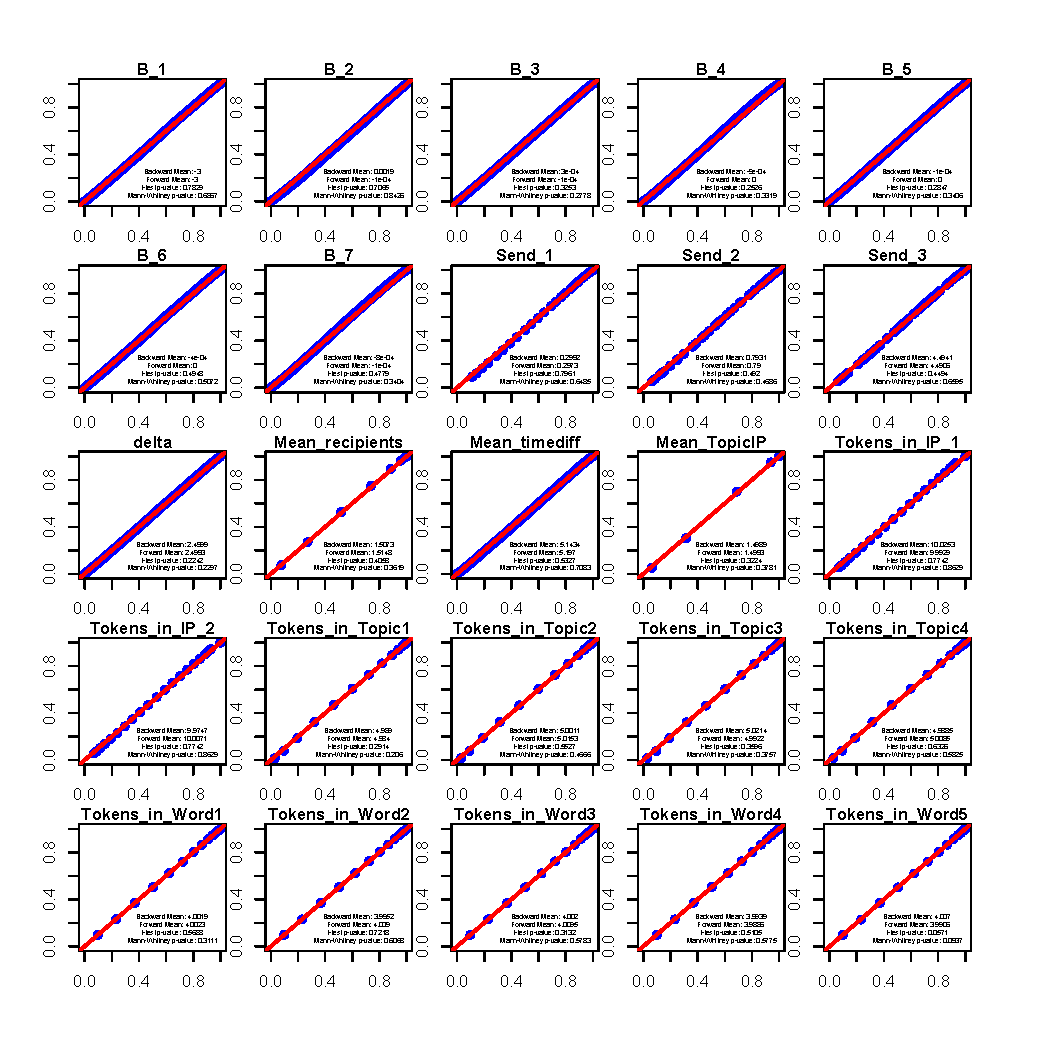
\includegraphics[width=1.05\textwidth]{Rplot.pdf} 
	\label{fig:GiR}
	\caption{Getting it Right test result}
\end{figure}
\begin{figure}[H]
	\centering
	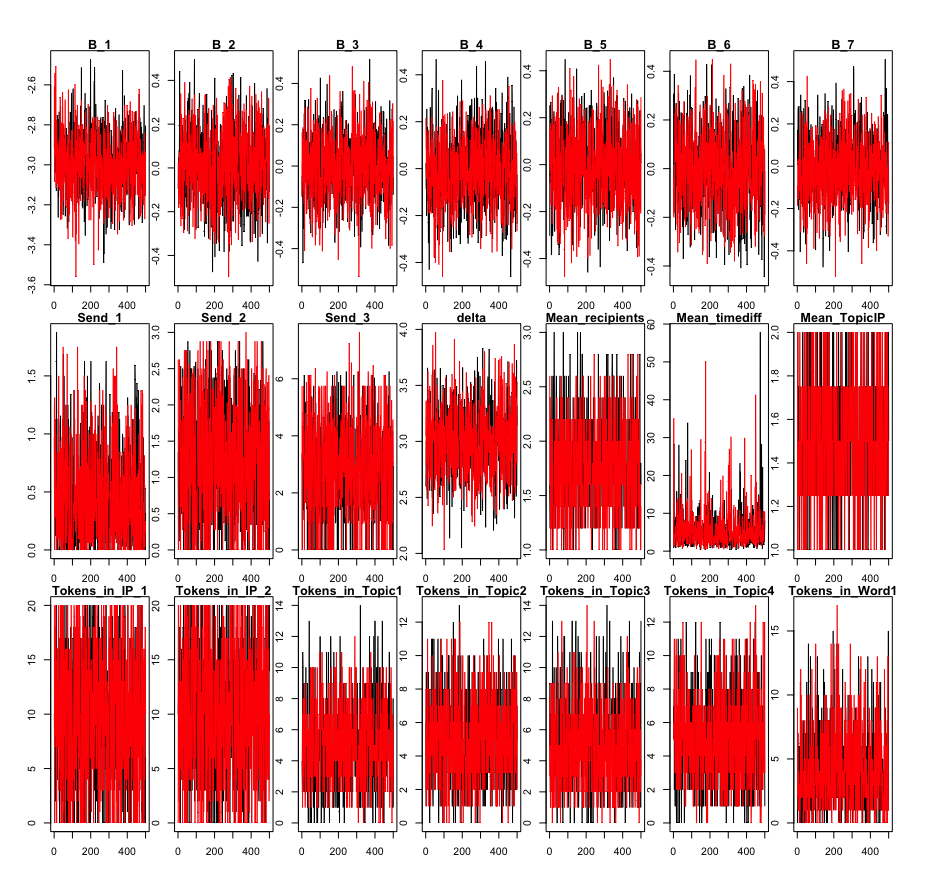
\includegraphics[width=1.05\textwidth]{trace.png} 
	\label{fig:GiRtrace}
	\caption{Getting it Right test traceplot (Black- Forward and Red - Backward)}
\end{figure}
 \section{Appliction to North Carolina email data}  \label{sec: Application to North Carolina email data}
 To see the applicability of the model, we used the North Carolina email data using two counties, Vance county and Dare county, which are the two counties whose email corpus cover the date of Hurricane Sandy (October 22, 2012 – November 2, 2012). Especially, Dare county geographically covers the Outer Banks, so we would like to see how the communication pattern changes during the time period surrounding Hurricane Sandy. Here we apply IPTM to both data and demonstrate the effectiveness of the model at predicting and explaining continuous-time textual communications.
 \subsection{Vance county email data} \label{subsec: Vance county email data}
Vance county data contains $D=185$ emails sent between $A=18$ actors, including $W=620$ vocabulary in total. We used $K=5$ topics and $C=2$ interaction patterns. MCMC sampling was implemented based on the order and scheme illustrated in Section \ref{sec: Inference}. We set the outer iteration number as $I=500$, the inner iteration numbers as $n_1=1, n_2=1,$ and $n_3=3300$. First 50 outer iterations and first 300 iterations of third inner iteration were used as a burn-in, and every $20^{th}$ sample was taken as a thinning process of third inner iteration. In addition, after some experimentation, $\sigma_Q^2$ was set as 0.2, to ensure sufficient acceptance rate. MCMC diagnostic plots are attached in APPENDIX D, as well as the geweke test statistics. \\\newline
 Below are the summary of IP-topic-word assignments. Each interaction pattern is paired with (a) posterior estimates of dynamic network effects $\boldsymbol{b}^{(c)}$ corresponding to the interaction pattern, and (b) the top 10 most likely words to be generated conditioned on the topic and their corresponding interaction pattern.
 \begin{figure}[ht]
 	\centering
 	 	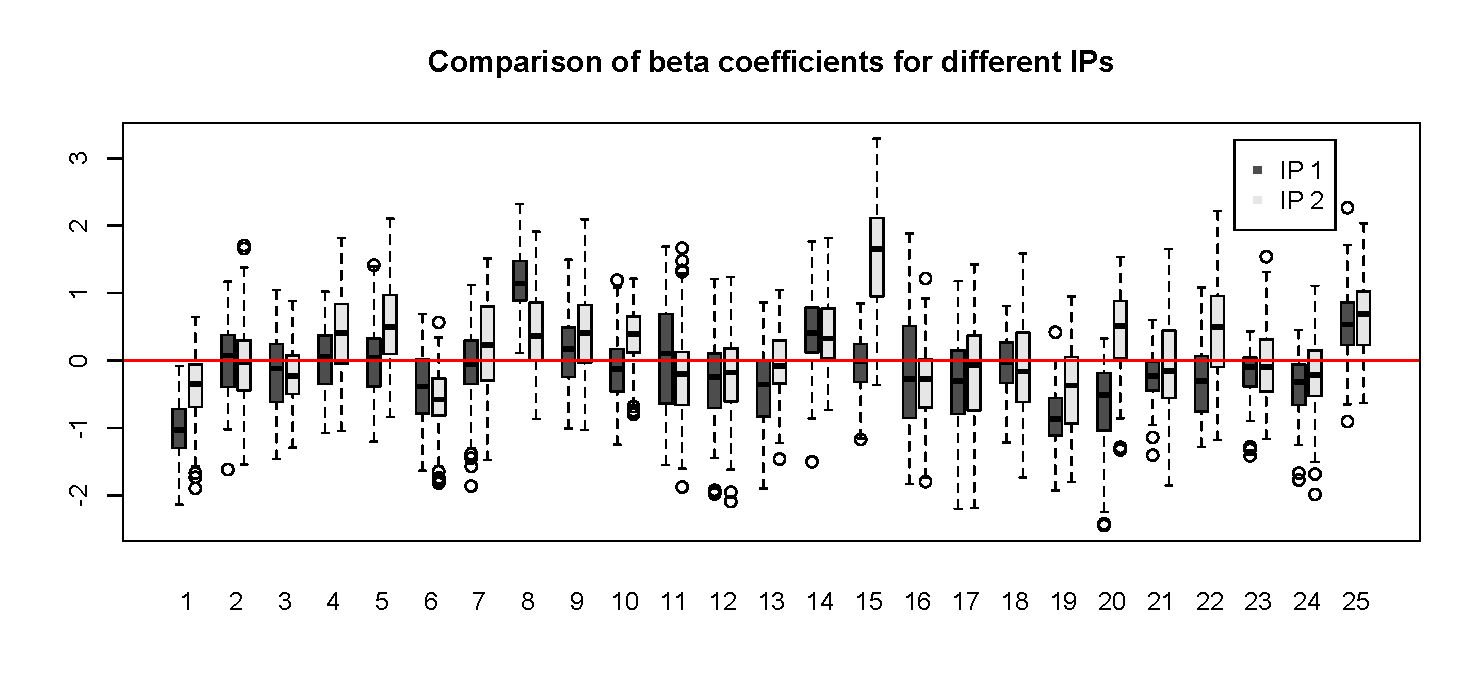
\includegraphics[width=1\textwidth]{betaplot.pdf} 
 	\caption{Posterior distribution of  $\boldsymbol{b}^{(c)}$ for Vance county emails}
 	\label{fig:Vanceboxplot}
 \end{figure}
 \begin{table}[ht]
 	\centering
 	\begin{tabular}{|l|l|l|l|l|l|l|l|l|l|}
 		\hline
 		covariate & 1&2 - 4&5 - 7& 8 - 10 & 11 - 13 & 14 - 16& 17 - 19 & 20 - 22&23 - 25\\
 	\hline	name & intercept & outdegree & indegree & send & receive & 2-send & 2-receive & sibling & cosibling\\
 	 		\hline
 	\end{tabular}
 	\caption {Network statistics}
 \end{table}
 \normalsize
By examining the estimates in Figure 2 and their corresponding interpretation, it seems that there exist strong effects of dynamic network covariates. That is, whether the sender and receiver previously had dyadic or triangle interaction strongly increase the rate of their interactions. \textcolor{red}{What are the findings here?}\newpage
 \begin{figure}[ht]
 	\centering
 		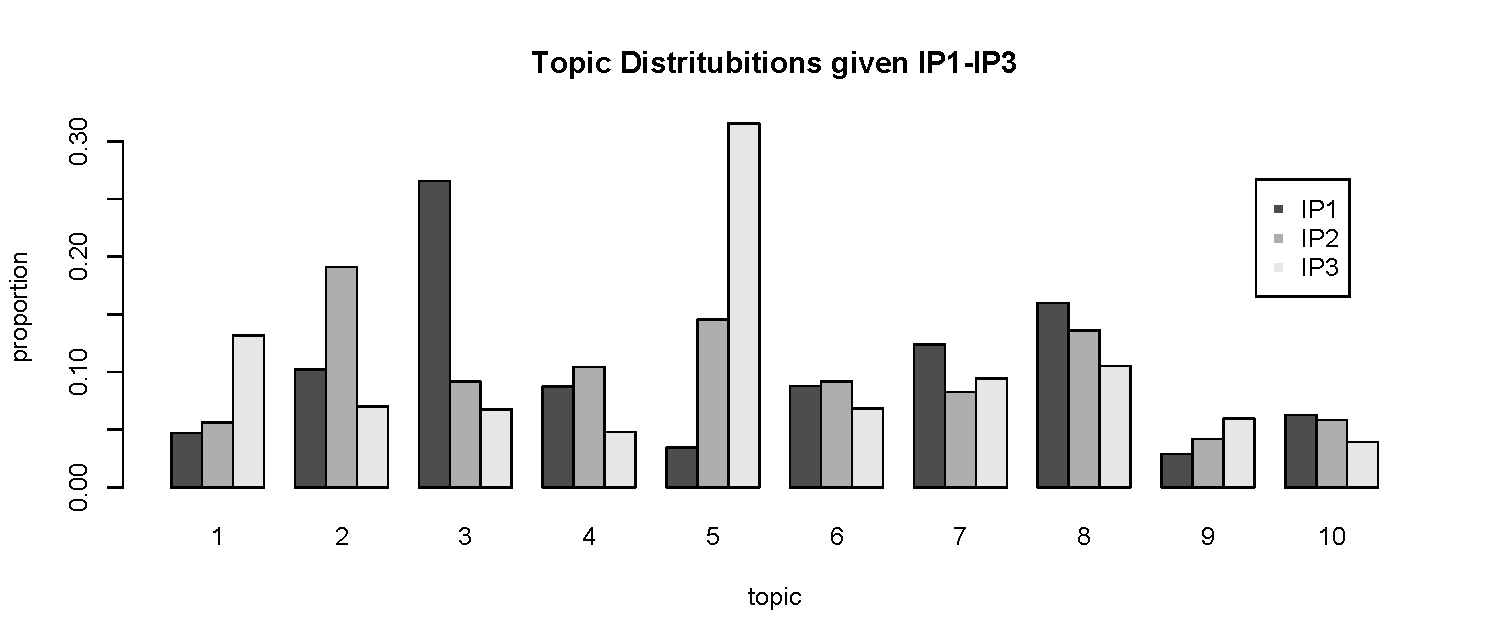
\includegraphics[width=0.7\textwidth]{topicplot.pdf} 
 	\caption{Posterior distribution of $\mathcal{Z}$ for Vance county emails}
 	\label{fig:Vancebarplot}
 \end{figure} 
\noindent Next, we scrutinize the topic distributions in Figure 3. There is some distinctive differences in the topic distributions $\mathcal{Z}$, given the assignment of interaction patterns to the documents $\mathcal{C}$. Specifically, each interaction pattern has different topics as the topic with highest probability.
 \normalsize
 \newline
 Furthermore, we look at the distribution of words given the topics, which corresponds to Algorithm 4 in the generative process. Since the topic-word distribution $\phi$ does not depend on the interaction patterns as previous cases, Table 3 lists top 10 topics with top 10 words that have the highest probability conditioned on the topic. In addition, this time we try to check the interaction pattern-word distribution by listing top 10 words that have the highest probability conditioned on the interaction pattern. It seems that the words are not significantly different, having several words like `director', `phones', `department', `description', or `henderson' (county seat of Vance county) appeared repetitively across the most of the topics or interaction patterns. The word 'will' was ranked the top in most of the lists, probably because it was not deleted during the text mining process while other similar type of words like `am', `is', `are', or `can' are all removed. \\
 \begin{table}[ht]
 	\centering
 	\begin{tabular}{|l||l||}
 		\hline
 		{\textbf{IP1} }&{\textbf{IP2} }\\
 		\hline\hline
 		K=5, K=2 & K=3, K=4, K=1\\
 		\hline
 	operations, description&emergency, electronic, will\\
 	emergency, phase & operations, message, meeting\\
 	henderson, planning& fax, request, director\\
 	director, development & henderson, review, phone\\
 	street, director & street, response, october\\
 	church, henderson& center, records, extension\\
 	suite, fax & director, manager, phones\\
 	office, church & church, pursuant, latest\\ 
 	center, phone & office, ncgs, directory\\
 	communications, email & communications, chapter, attached\\
 		\hline
 	\end{tabular}
 	\caption {Summary of top 10 words that have the highest probability conditioned on the topic}
 	\label{table:VancewordsMCMC}
 \end{table}
 \subsection{Dare county email data} \label{subsec: Dare county email data}
 Dare county data contains $D=2247$ emails between $A=27$ actors, including $W=2907$ vocabulary in total. Again, we used $K=10$ topics and $C=3$ interaction patterns. MCMC sampling was implemented based on the order and scheme illustrated earlier. We set the outer iteration number as $I=1000$, and inner iteration numbers as $n_1=3, n_2=3,$ and $n_3=3300$. In addition, after some experimentation, $\sigma^2_Q$ was set as 0.02, to ensure sufficient acceptance rate. In our case, the average acceptance rate for $\boldsymbol{b}$ was 0.277. As demonstrated in Algorithm 5, the last value of $\mathcal{C}$, the last value of $\mathcal{Z}$, and the last $n_3$ length chain of $\mathcal{B}$ were taken as the final posterior samples. Among the $\mathcal{B}$ samples, 300 were discarded as a burn-in and every $10^{th}$ samples were taken. After these post-processing, MCMC diagnostic plots are attached in APPENDIX D, as well as geweke test statistics. 
\bibliographystyle{apalike}
\bibliography{IPTM}
\newpage
\appendix
 \section*{APPENDIX}
 \renewcommand{\thesubsection}{\Alph{subsection}}
 \iffalse
 \subsection{Notations in IPTM}\label{subsec: notations}
  \begin{table}[ht]
  	\centering
  	\scalebox{0.9}{ 	\begin{tabular}{ |c|c|c|} 
  			\hline
  			\hline
  			  			Sender of the $d^{th}$ document&$i^{(d)}$ & Scalar\\
  			  			\hline 
  	  			Receivers of the $d^{th}$ document&$J^{(d)}$ & $|J^{(d)}|$-dimensional vector\\
  	  			\hline 
  	  			Individual receiver of the $d^{th}$ document&$j^{(d)}$ & Scalar\\
  	  			\hline
  			  Time of the $d^{th}$ document&$t^{(d)}$ & Scalar\\
  			  			\hline 			
  			Authors of the corpus &$\mathcal{A}$ & Set\\
  			\hline
  			Number of authors &$A$ & Scalar \\
  			\hline
  			Number of documents &$D$ & Scalar \\
  			\hline
  			Number of words in the $d^{th}$ document &$N^{(d)}$ & Scalar \\
  			\hline
  			Number of topics & $K$ & Scalar \\
  			\hline
  			Vocabulary size & $W$ & Scalar \\
  			\hline
  			Number of interaction patterns &$C$ & Scalar \\
  			\hline
  			Number of words assigned to word and topic&$N^{WK}$ & Scalar \\
  			\hline
  			Interaction pattern of the $k^{th}$ topic&$C_k$ & Scalar\\
  			\hline 
  			Tuning parameter in tie generative process& $\delta$ & Scalar\\
  			\hline 
  			Poisson parameter for number of words $N^{(d)}$& $\zeta$ & Scalar\\ \hline
  			Words in the $d^{th}$ document&$\boldsymbol{w}^{(d)}$ & $N^{(d)}$-dimensional vector\\
  			\hline 
  			$n^{th}$ word in the $d^{th}$ document&${w}_n^{(d)}$ & $n^{th}$  component of $\boldsymbol{w}^{(d)}$\\
  			\hline 	
  			Topic assignments in the $d^{th}$ document&$\boldsymbol{z}^{(d)}$ & $N^{(d)}$-dimensional vector\\
  			\hline 
  			Topic assignments for $n^{th}$ word in the $d^{th}$ document&${z}_n^{(d)}$ & $n^{th}$ component of $\boldsymbol{z}^{(d)}$\\
  			\hline 	
  			Dirichlet concentration prior for document topic distribution&$\alpha$ & Scalar \\
  			\hline	
  			Dirichlet base prior for document topic distribution&$\boldsymbol{m}$ & $K$-dimensional vector \\
  			\hline			
  			Dirichlet concentration prior for topic word distribution&$\beta$ & Scalar \\
  			\hline			 
  			Dirichlet base prior for topic word distribution&$\boldsymbol{u}$ & $W$-dimensional vector  \\
  			\hline				 	
  			Variance of Normal prior&$\sigma^2$ & Scalar \\
  			\hline		
  			Probabilities of the words given topic $k$ &$\boldsymbol{\phi}^{(k)}$ & $W$-dimensional vector\\
  			\hline
  			Probabilities of the topics given the $d^{th}$ document &$\boldsymbol{\theta}^{(d)}$ & $K$-dimensional vector\\
  			\hline		
  			Coefficient of the intensity process given interaction pattern $c$ &$\boldsymbol{b}^{(c)}$ & $p$-dimensional vector\\
  			\hline		
  			Network statistics for $(i, j)$ at time $t$ given interaction pattern $c$ &$\boldsymbol{x}^{(c)}_t{(i,j)}$ & $p$-dimensional vector\\
  			\hline		
  			Stochastic intensity of document $d$ at time $t$ & $\boldsymbol{\lambda}^{(d)}(t)$ & $A\times A$ matrix\\
  			\hline
  		  	Stochastic intensity of $(i, j)$ in document $d$ at time $t$ & ${\lambda}_{ij}^{(d)}(t)$ & Scalar\\
  		  	\hline	
  		  	  		  	Proportion of topics in document $d$ corresponding to interaction pattern $c$ & $p_c^{(d)}$ & Scalar\\
  		  	  		  	\hline
  		  Time increments associated to $(i, J)$ pair & $\Delta T_{iJ}$ & Scalar\\
  		  		\hline
  			\hline
  		\end{tabular}}
  		\caption {Symbols associated with IPTM, as used in this paper}
  		\label{table:SymbolsIPTM}
  	\end{table}
  	\normalsize
  	\fi
  	 \subsection{Normalizing constant of non-empty Gibbs measure}\label{subsec: non-empty Gibbs measure}
  	 In Section \ref{subsec: Tie Generating Process}, we define the non-empty Gibbs measure such that 
 the probability of sender $i$ selecting the binary receiver vector of length $(A-1)$, $J_i^{(d)}$ is given by
  	 \begin{equation*} \text{P}(J_i^{(d)}) = \frac{1}{Z(\delta,\mbox{log}(\lambda_i^{(d)}))} \exp\Big\{ \mbox{log}\big(\text{I}( \sum_{j \in \mathcal{A}_{\backslash i}} J^{(d)}_{ij} > 0 )\big) + \sum_{j \in \mathcal{A}_{\backslash i}} (\delta+\mbox{log}(\lambda_{ij}^{(d)}))J_{ij}^{(d)} \Big\}.
  	 \end{equation*}
  	 	 To use this distribution efficiently, we need to derive a closed-form expression for $Z(\delta,\mbox{log}(\lambda_{i}^{(d)}))$ that does not require brute-force summation over the support of $J_i^{(d)}$. We begin by recognizing that if $J_i^{(d)}$ were drawn via independent Bernoulli distributions in which P($J_{ij}^{(d)}$=1) was given by logit$\left(\delta+\lambda_{ij}^{(d)}\right)$, then \begin{equation*}\text{P}(J_i^{(d)}) \propto \exp\Big\{  \sum_{j \in \mathcal{A}_{\backslash i}} (\delta+\mbox{log}(\lambda_{ij}^{(d)}))J_{ij}^{(d)}\Big\}.  	 \end{equation*}
  	 	  This is straightforward to verify by looking at 
  	 	  \begin{equation*}
  	 	  \begin{aligned}\text{P}(J_{ij}^{(d)}=1|J_{i,-j})&=\frac{ \exp{(\delta+\mbox{log}(\lambda_{ij}^{(d)}))}\exp\Big\{ \sum_{h\neq i,j} (\delta+\mbox{log}(\lambda_{ih}^{(d)}))J_{ih}^{(d)} \Big\}}{\exp{(\delta+\mbox{log}(\lambda_{ij}^{(d)}))}\exp\Big\{   \sum_{h\neq i,j} (\delta+\mbox{log}(\lambda_{ih}^{(d)}))J_{ih}^{(d)} \Big\}+ \exp{(0)}\exp\Big\{ \sum_{h\neq i,j} (\delta+\mbox{log}(\lambda_{ih}^{(d)}))J_{ih}^{(d)} \Big\}},\\
  	 	  &=\frac{ \exp{(\delta+\mbox{log}(\lambda_{ij}^{(d)}))}}{\exp{(\delta+\mbox{log}(\lambda_{ij}^{(d)}))} + 1}.\end{aligned}\end{equation*}
  	 	  We denote the logistic-Bernoulli normalizing constant as $Z^{l}(\delta,\lambda_i^{(d)})$, which is defined as 
  	 	  \begin{equation*}
  	 	  Z^{l}(\delta,\mbox{log}(\lambda_{i}^{(d)}))=\sum_{J_i \in [0,1]^{(A-1)}} \exp\Big\{\sum_{j\neq i} (\delta+\mbox{log}(\lambda_{ij}^{(d)}))J_{ij}^{(d)} \Big\}.
  	 	  \end{equation*}
  	 
  	 Now, since 
  	\begin{equation*}
  	\exp\Big\{ \mbox{log}\big(\text{I}( \sum_{j \in \mathcal{A}_{\backslash i}} J_{ij} > 0 )\big) + \sum_{j \in \mathcal{A}_{\backslash i}} (\delta+\mbox{log}(\lambda_{ij}^{(d)}))J_{ij}^{(d)} \Big\}= \exp\Big\{ \sum_{j \in \mathcal{A}_{\backslash i}} (\delta+\mbox{log}(\lambda_{ij}^{(d)}))J_{ij}^{(d)} \Big\},
  	\end{equation*} except when $\sum\limits_{j \in \mathcal{A}_{\backslash i}} J^{(d)}_{ij}=0$, in which case the left-hand side 
  	\begin{equation*}
\exp\Big\{ \mbox{log}\big(\text{I}( \sum_{j \in \mathcal{A}_{\backslash i}} J_{ij} > 0 )\big) + \sum_{j \in \mathcal{A}_{\backslash i}} (\delta+\mbox{log}(\lambda_{ij}^{(d)}))J_{ij}^{(d)} \Big\}= 0.  	
\end{equation*}
 As such, we note that 
 \begin{equation*}
 \begin{aligned}
Z(\delta,\mbox{log}(\lambda_{i}^{(d)}))& = Z^{l}(\delta,\mbox{log}(\lambda_{i}^{(d)})) -  \exp\Big\{ \sum\limits_{\substack{j \in \mathcal{A}_{\backslash i}, J^{(d)}_{ij}=0}} (\delta+\mbox{log}(\lambda_{ij}^{(d)}))J_{ij}^{(d)} \Big\}
\\& = Z^{l}(\delta,\mbox{log}(\lambda_{i}^{(d)})) -  1.
\end{aligned}
 \end{equation*}
   We can therefore derive a closed form expression for $Z(\delta,\mbox{log}(\lambda_{i}^{(d)}))$ via a closed form expression for $Z^{l}(\delta,\mbox{log}(\lambda_{i}^{(d)}))$. This can be done by looking at the probability of the zero vector under the logistic-Bernoulli model:
   \begin{equation*}
   \begin{aligned}
\frac{\exp\Big\{\sum_{j\neq i, J^{(d)}_{ij}=0} (\delta+\mbox{log}(\lambda_{ij}^{(d)}))J_{ij}^{(d)} \Big\}}{Z^{l}(\delta,\mbox{log}(\lambda_{ij}^{(d)}))} &= \prod_{j \in \mathcal{A}_{\backslash i} }   \frac{ \exp\{(-(\delta+\mbox{log}(\lambda_{ij}^{(d)})))\}}{\exp\{(-(\delta+\mbox{log}(\lambda_{ij}^{(d)})))\} + 1},\\
\frac{1}{Z^{l}(\delta,\mbox{log}(\lambda_{ij}^{(d)}))} &= \prod_{j \in \mathcal{A}_{\backslash i} }   \frac{ \exp{(-(\delta+\mbox{log}(\lambda_{ij}^{(d)})))}}{\exp{(-(\delta+\mbox{log}(\lambda_{ij}^{(d)})))} + 1}, \\
Z^{l}(\delta,\mbox{log}(\lambda_{ij}^{(d)})) &= \frac{1}{\prod_{j \in \mathcal{A}_{\backslash i}}   \frac{ \exp{(-(\delta+\mbox{log}(\lambda_{ij}^{(d)})))}}{\exp{(-(\delta+\mbox{log}(\lambda_{ij}^{(d)})))} + 1}}.
  	 \end{aligned}  
  	 \end{equation*}
  	 The closed form expression for the normalizing constant under the non-empty Gibbs measure is therefore    \begin{equation*}
  	 \begin{aligned}Z(\delta,\lambda_i^{(d)}) = \Big(\prod_{j \in \mathcal{A}_{\backslash i}} \Big(\mbox{exp}\{\delta+\mbox{log}(\lambda_{ij}^{(d)})\} + 1\Big)\Big)-1.
  	  \end{aligned}  
  	  \end{equation*}
  \subsection{Integrating out $\Phi$ and $\Theta$ in latent Dirichlet allocation}\label{subsec: phitheta integration}
  \begin{equation*}
  \begin{aligned}
   &  P(\Phi, \Theta, \mathcal{Z}, \mathcal{C}, \mathcal{B}, \delta, \mathcal{W}, \mathcal{J}_{\mbox{a}}, \mathcal{I}_{\mbox{o}}, \mathcal{J}_{\mbox{o}}, \mathcal{T}_{\mbox{o}}| \beta, \boldsymbol{u}, \alpha, \boldsymbol{m}, \mu_{\boldsymbol{b}}, \Sigma_{\boldsymbol{b}}, \mu_\delta, \sigma^2_\delta) \\& 
   \propto P( \mathcal{Z}, \mathcal{C}, \mathcal{B},  \delta, \mathcal{W}, \mathcal{J}_{\mbox{a}}, \mathcal{I}_{\mbox{o}}, \mathcal{J}_{\mbox{o}}, \mathcal{T}_{\mbox{o}}|\Phi, \Theta, \mu_{\boldsymbol{b}}, \Sigma_{\boldsymbol{b}}, \mu_\delta, \sigma^2_\delta)P(\Phi, \Theta| \beta, \boldsymbol{u}, \alpha, \boldsymbol{m})
   \\& 
 \propto P(\mathcal{Z}|\mathcal{W},\Theta)P(\mathcal{C})P(\mathcal{B}|\mathcal{C}, \mu_{\boldsymbol{b}}, \Sigma_{\boldsymbol{b}})P(\delta|\mu_\delta, \sigma^2_\delta)P(\mathcal{W}|\Phi)P(\Phi| \beta, \boldsymbol{u})P(\Theta|\alpha, \boldsymbol{m})P(\mathcal{J}_{\mbox{a}}, \mathcal{I}_{\mbox{o}}, \mathcal{J}_{\mbox{o}}, \mathcal{T}_{\mbox{o}} |\mathcal{Z}, \mathcal{C}, \mathcal{B}, \delta)
  \\&=\Big[\prod_{d=1}^{D}\prod_{n=1}^{N^{(d)}} P( z_n^{(d)}|w_n^{(d)},  \boldsymbol{\theta}^{(d)})\Big]\times \Big[\prod_{k=1}^{K} P(C_k)\Big] \times\Big[\prod_{c=1}^{C} P( \boldsymbol{b}^{(c)}| \mu_{\boldsymbol{b}}, \Sigma_{\boldsymbol{b}})\Big] \times P(\delta|\mu_\delta, \sigma^2_\delta)\\&\quad \quad\times \Big[\prod_{d=1}^{D}\prod_{n=1}^{N^{(d)}} P(w_n^{(d)}| \phi_{z_n^{(d)}})\Big]\times \Big[\prod_{k=1}^{K} P( \boldsymbol{\phi}^{(k)}| \beta, \boldsymbol{u})\Big]\times \Big[\prod_{d=1}^{D} P( \boldsymbol{\theta}^{(d)}|\alpha, \boldsymbol{m})\Big]\\&\quad \quad\quad \quad\times\Big[\prod_{d=1}^{D} P(\mathcal{J}^{(d)}_{\mbox{a}}, i^{(d)}_{\mbox{o}}, J^{(d)}_{\mbox{o}}, t^{(d)}_{\mbox{o}} |\mathcal{I}^{(<d)}_{\mbox{o}}, \mathcal{J}^{(<d)}_{\mbox{o}}, \mathcal{T}^{(<d)}_{\mbox{o}},\mathcal{Z}, \mathcal{C}, \mathcal{B}, \delta)\Big] 
  \end{aligned}
  \end{equation*}
  Dropping the terms independent of tokens out, we can simplify as below:
  \begin{equation*}
  \begin{aligned}
  & \propto \Big[\prod_{d=1}^{D}\prod_{n=1}^{N^{(d)}} P(z_n^{(d)}|w_n^{(d)},  \boldsymbol{\theta}^{(d)})\Big]\times\Big[\prod_{d=1}^{D}\prod_{n=1}^{N^{(d)}} P(w_n^{(d)}| \phi_{z_n^{(d)}})\Big]\times \Big[\prod_{k=1}^{K} P( \boldsymbol{\phi}^{(k)}| \beta, \boldsymbol{u})\Big] \times\Big[\prod_{d=1}^{D} P( \boldsymbol{\theta}^{(d)}|\alpha, \boldsymbol{m})\Big] \\&
  \propto\Big[\prod_{d=1}^{D}\prod_{n=1}^{N^{(d)}} \phi_{w_n^{(d)}z_n^{(d)}}\Big]\times \Big[\prod_{d=1}^{D}\prod_{n=1}^{N^{(d)}} \boldsymbol{\theta}^{(d)}_{z_n^{(d)}}\Big]\\&\quad\quad \times \Big[\prod_{k=1}^{K} \Big(\frac{\Gamma(\sum_{w=1}^{W}\beta u_w)}{\prod_{w=1}^{W}\Gamma(\beta u_w)}\prod_{w=1}^{W}\phi_{wk}^{\beta u_w-1} \Big)\Big]\times \Big[\prod_{d=1}^{D} \Big(\frac{\Gamma(\sum_{k=1}^{K}\alpha m_k)}{\prod_{k=1}^{K}\Gamma(\alpha m_k)}\prod_{k=1}^{K}(\boldsymbol{\theta}^{(d)}_{k})^{\alpha m_k-1} \Big)\Big] \\&
  \propto\Big[\frac{\Gamma(\sum_{w=1}^{W}\beta u_w)}{\prod_{w=1}^{W}\Gamma(\beta u_w)}\Big]^K \times \prod_{d=1}^{D} \Big[\frac{\Gamma(\sum_{k=1}^{K}\alpha m_k)}{\prod_{k=1}^{K}\Gamma(\alpha m_k)}\Big]\times
  \Big[\prod_{k=1}^{K}\prod_{w=1}^{W}\phi_{wk}^{N^{WK}_{wk}+\beta u_w-1}\Big]\times\Big[\prod_{d=1}^{D}\prod_{k=1}^{K}(\boldsymbol{\theta}^{(d)}_{k})^{N_{k|d}+\alpha m_k-1}\Big]
  \end{aligned}
  \end{equation*}
  where $N^{WK}_{wk}$ is the number of times the $w^{th}$ word in the vocabulary is assigned to topic $k$, and $N_{k|d}$ is the number of times topic k shows up in the document $d$. We can integrate out the random variables $\Theta$ and $\Phi$, making use of the fact that the Dirichlet distribution is a conjugate prior of multinomial distribution. Applying the well-known formula $\int\prod_{n=1}^{M}[x_m^{k_m-1}dx_m]=\frac{\prod_{n=1}^M\Gamma(k_m)}{\Gamma(\sum_{n=1}^Mk_m)}$, we have:
  \begin{equation*}
  \begin{aligned}
  &P(\mathcal{Z}, \mathcal{C}, \mathcal{B},\delta, \mathcal{W},\mathcal{J}_{\mbox{a}}, \mathcal{I}_{\mbox{o}}, \mathcal{J}_{\mbox{o}}, \mathcal{T}_{\mbox{o}}| \beta, \boldsymbol{u}, \alpha, \mu_{\boldsymbol{b}}, \Sigma_{\boldsymbol{b}}, \mu_\delta, \sigma^2_\delta)\\&=\mbox{Const.}\int_{\Theta}\int_{\Phi}\Big[\prod_{k=1}^{K}\prod_{w=1}^{W}\phi_{wk}^{N^{WK}_{wk}+\beta u_w-1}\Big]\Big[\prod_{d=1}^{D}\prod_{k=1}^{K}(\boldsymbol{\theta}^{(d)}_{k})^{N_{k|d}+\alpha m_k-1}\Big]d\Phi d\Theta
  \\&=\mbox{Const.}\Big[\prod_{k=1}^{K}\int_{\phi_{:k}}\prod_{w=1}^{W}\phi_{wk}^{N^{WK}_{wk}+\beta u_w-1  }d\phi_{:k}\Big]\times\Big[\prod_{d=1}^{D}\int_{\theta_{:d}}\prod_{k=1}^{K}(\boldsymbol{\theta}^{(d)}_{k})^{N_{k|d}+\alpha m_k-1}d\theta_{:d}\Big]
  \\&=\mbox{Const.}\Big[\prod_{k=1}^{K}\frac{\prod_{w=1}^W\Gamma(N_{wk}^{WK}+\frac{\beta}{W})}{\Gamma(\sum_{w=1}^WN_{wk}^{WK}+\beta )}\Big]\times\Big[\prod_{d=1}^{D}\frac{\prod_{k=1}^K\Gamma(N_{k|d}+\alpha m_k)}{\Gamma(N_{\cdot|d}+\alpha)}\Big].
  \end{aligned}
  \end{equation*}
  \subsection{Conditional probability of $\mathcal{Z}$} \label{subsec: conditional probability Z}
  \begin{equation*}
  \begin{aligned}
  & P(\boldsymbol{w}^{(d)}, \boldsymbol{z}^{(d)}|\mathcal{W}_{\backslash d}, \mathcal{Z}_{\backslash d}, \beta, \boldsymbol{u}, \alpha, \boldsymbol{m}) \\& \propto \prod_{n=1}^{N^{(d)}}P(z^{(d)}_n=k, w^{(d)}_n=w| \mathcal{W}_{\backslash d, n}, \mathcal{Z}_{\backslash d, n}, \beta, \boldsymbol{u}, \alpha, \boldsymbol{m})
  \end{aligned}
  \end{equation*} 
  To obtain the Gibbs sampling equation, we need to obtain an expression for $P(z^{(d)}_n=k,  w^{(d)}_n=w|\mathcal{W}_{\backslash d, n}, \mathcal{Z}_{\backslash d, n}, \beta, \boldsymbol{u}, \alpha, \boldsymbol{m})$,
  From Bayes' theorem and Gamma identity $\Gamma(k+1)=k\Gamma(k)$,
  \begin{equation*}
  \begin{aligned}
  & P(z^{(d)}_n=k, w^{(d)}_n=w|\mathcal{W}_{\backslash d, n}, \mathcal{Z}_{\backslash d, n}, \beta, \boldsymbol{u}, \alpha, \boldsymbol{m}) \\& \propto 
  \frac{P(\mathcal{W}, \mathcal{Z}|\beta, \boldsymbol{u}, \alpha, \boldsymbol{m})}{P(\mathcal{W}_{\backslash d, n}, \mathcal{Z}_{\backslash d, n}|\beta, \boldsymbol{u}, \alpha, \boldsymbol{m})}\\& \propto \frac{\prod_{k=1}^{K}\frac{\prod_{w=1}^W\Gamma(N_{wk}^{WK}+\beta u_w)}{\Gamma(\sum_{w=1}^WN_{wk}^{WK}+\beta )}\times\prod_{k=1}^K\frac{\Gamma(N_{k|d}+\alpha m_k)}{\Gamma(N_{\cdot|d}+\alpha)}}{\prod_{k=1}^{K}\frac{\prod_{w=1}^W\Gamma(N_{wk, \backslash d, n}^{WK}+\beta u_w)}{\Gamma(\sum_{w=1}^WN_{wk, \backslash d, n}^{WK}+\beta )}\times\prod_{k=1}^K\frac{\Gamma(N_{k|d, \backslash d, n}+\alpha m_k)}{\Gamma(N_{\cdot|d, \backslash d, n}+\alpha)}}\\ & \propto 
  \frac{N_{wk, \backslash d, n}^{WK}+\frac{\beta}{W}}{\sum_{w=1}^WN_{wk,  \backslash d, n}^{WK}+\beta}\times\frac{N_{k|d, \backslash d, n}+\alpha m_k}{N^{(d)}-1+\alpha}
  \end{aligned}
  \end{equation*}
  Then, same as for LDA, we also know that the topic assignment $z_n^{(d)}=k$ is obtained by:
  \begin{equation*}
  \begin{aligned}
  &P(z^{(d)}_n=k|w^{(d)}_n=w, \mathcal{W}_{\backslash d, n}, \mathcal{Z}_{\backslash d,n}, \beta, \boldsymbol{u}, \alpha, \boldsymbol{m}) \propto
  \frac{N_{k|d, \backslash d, n}+\alpha m_k}{N^{(d)}-1+\alpha}
  \end{aligned}
  \end{equation*}
  In addition, the conditional probability that a new word generated in the document would be $w_n^{(d)}=w$, given that it is generated from topic $z_n^{(d)}=k$ is obtained by:
  \begin{equation*}
  \begin{aligned}
  & P(w^{(d)}_m=w|z^{(d)}_m=k, \mathcal{W}_{\backslash d, n}, \mathcal{Z}_{\backslash d, nm}, \beta, \boldsymbol{u}, \alpha, \boldsymbol{m}) \propto 
  \frac{N_{wk, \backslash d, n}^{WK}+\frac{\beta}{W}}{\sum_{w=1}^WN_{wk, \backslash d, n}^{WK}+\beta}
  \end{aligned} 
  \end{equation*}
  \iffalse
  NOTE: Using Equation (28), the unnormalized constant we use to check the model convergence and the corresponding log-constant is,
  \begin{equation*}
  \begin{aligned}
  & \prod_{d=1}^{D}\prod_{n=1}^{N^{(d)}}  P(z^{(d)}_n=k, w^{(d)}_n=w|\mathcal{W}_{\backslash d, n}, \mathcal{Z}_{\backslash d,m}, \beta, \boldsymbol{u}, \alpha, \boldsymbol{m}) \\ & \propto \prod_{d=1}^{D}\prod_{n=1}^{N^{(d)}} 
  \frac{N_{w^{(d)}_nz^{(d)}_n, \backslash d, n}^{WK}+\frac{\beta}{W}}{\sum_{w=1}^WN_{wz^{(d)}_n,  \backslash d, n}^{WK}+\beta}\times\frac{N_{k|d, \backslash d, n}+\alpha m_{z^{(d)}_n}}{N^{(d)}-1+\alpha},
  \end{aligned}
  \end{equation*}
  \begin{equation*}
  \begin{aligned}
  & \sum_{d=1}^{D}\sum_{n=1}^{N^{(d)}} \mbox{log}\Big( P(z^{(d)}_n=k, w^{(d)}_n=w|\mathcal{W}_{\backslash d, n}, \mathcal{Z}_{\backslash d, n}, \beta, \boldsymbol{u}, \alpha, \boldsymbol{m})\Big) \\ & \propto \sum_{d=1}^{D}\sum_{n=1}^{N^{(d)}} 
  \mbox{log}\Big(N_{w^{(d)}_mz^{(d)}_m, \backslash d, n}^{WK}+\frac{\beta}{W}\Big)-\mbox{log}\Big(\sum_{w=1}^WN_{wz^{(d)}_m,  \backslash d, n}^{WK}+\beta\Big)\\&+\mbox{log}\Big(N_{k|d, \backslash d, n}+\alpha m_{z^{(d)}_m}\Big)-\mbox{log}\Big(N^{(d)}-1+\alpha\Big)
  \end{aligned}
  \end{equation*}
  \fi
  \end{document}

